\UseRawInputEncoding
%DIF LATEXDIFF DIFFERENCE FILE
%DIF DEL ./old/compiled_v015.tex   Sat Jan 13 15:45:06 2024
%DIF ADD ./compiled.tex            Sat Jan 13 15:52:25 2024

%%%%%%%%%%%%%%%%%%%%%%%%%%%%%%%%%%%%%%%%%%%%%%%%%%%%%%%%%%%%%%%%%%%%%%%%%%%%%%%%
%% SETTINGS
%%%%%%%%%%%%%%%%%%%%%%%%%%%%%%%%%%%%%%%%%%%%%%%%%%%%%%%%%%%%%%%%%%%%%%%%%%%%%%%%
%% Columns
\documentclass[final,3p,times,twocolumn]{elsarticle}
%% Use the options 1p,twocolumn; 3p; 3p,twocolumn; 5p; or 5p,twocolumn
%% for a journal layout:
%% \documentclass[final,1p,times]{elsarticle}
%% \documentclass[final,1p,times,twocolumn]{elsarticle}
%% \documentclass[final,3p,times]{elsarticle}
%% \documentclass[final,3p,times,twocolumn]{elsarticle}
%% \documentclass[final,5p,times]{elsarticle}
%% \documentclass[final,5p,times,twocolumn]{elsarticle}
%% \documentclass[preprint,review,12pt]{elsarticle}

%% Image width
\newlength{\imagewidth}
\newlength{\imagescale}
%% preamble
\usepackage[english]{babel}
\usepackage[table]{xcolor} % For coloring tables
\usepackage{booktabs} % For professional quality tables
\usepackage{colortbl} % For coloring cells in tables
\usepackage{amsmath, amssymb} % For mathematical symbols and environments
\usepackage{amsthm} % For theorem-like environments
\usepackage{lipsum} % just for sample text
\usepackage{natbib}
\usepackage{graphicx}
\usepackage{indentfirst}
\usepackage{bashful}
\usepackage[margin=10pt,font=small,labelfont=bf,labelsep=endash]{caption}
\usepackage{graphicx}
\usepackage{calc}
\usepackage[T1]{fontenc} % [REVISED]
\usepackage[utf8]{inputenc} % [REVISED]
\usepackage{hyperref}
\usepackage{accsupp}
%% Line numbers
\linespread{1.1}
% \linenumbers
% Tables
\usepackage[pass]{geometry}
% \usepackage{geometry}
\usepackage{pdflscape}
\usepackage{csvsimple}
\usepackage{xltabular}
\usepackage{booktabs}
\usepackage{siunitx}
\usepackage{makecell}
\sisetup{round-mode=figures,round-precision=3}
\renewcommand\theadfont{\bfseries}
\renewcommand\theadalign{c}
\newcolumntype{C}[1]{>{\centering\arraybackslash}m{#1}}
\renewcommand{\arraystretch}{1.5}
\definecolor{lightgray}{gray}{0.95}

%% Diff
\usepackage{xcolor}
% Define commands for highlighting
% diff
\usepackage[most]{tcolorbox} % for boxes with transparency
% Define colors with transparency (opacity value)
\definecolor{GreenBG}{rgb}{0,1,0}
\definecolor{RedBG}{rgb}{1,0,0}
% Define tcolorbox environments for highlighting
\newtcbox{\greenhighlight}[1][]{%
  on line,
  colframe=GreenBG,
  colback=GreenBG!50!white, % 50% transparent green
  boxrule=0pt,
  arc=0pt,
  boxsep=0pt,
  left=1pt,
  right=1pt,
  top=2pt,
  bottom=2pt,
  tcbox raise base
}
\newtcbox{\redhighlight}[1][]{%
  on line,
  colframe=RedBG,
  colback=RedBG!50!white, % 50% transparent red
  boxrule=0pt,
  arc=0pt,
  boxsep=0pt,
  left=1pt,
  right=1pt,
  top=2pt,
  bottom=2pt,
  tcbox raise base
}
\newcommand{\REDSTARTS}{\color{red}}
\newcommand{\REDENDS}{\color{black}}
\newcommand{\GREENSTARTS}{\color{green}}
\newcommand{\GREENENDS}{\color{black}}
%%%%%%%%%%%%%%%%%%%%%%%%%%%%%%%%%%%%%%%%%%%%%%%%%%%%%%%%%%%%%%%%%%%%%%%%%%%%%%%%
%% JOURNAL NAME
%%%%%%%%%%%%%%%%%%%%%%%%%%%%%%%%%%%%%%%%%%%%%%%%%%%%%%%%%%%%%%%%%%%%%%%%%%%%%%%%
\journal{Heliyon}
%%%%%%%%%%%%%%%%%%%%%%%%%%%%%%%%%%%%%%%%%%%%%%%%%%%%%%%%%%%%%%%%%%%%%%%%%%%%%%%%
%% DOCUMENT STARTS
%%%%%%%%%%%%%%%%%%%%%%%%%%%%%%%%%%%%%%%%%%%%%%%%%%%%%%%%%%%%%%%%%%%%%%%%%%%%%%%%
%DIF PREAMBLE EXTENSION ADDED BY LATEXDIFF
%DIF UNDERLINE PREAMBLE %DIF PREAMBLE
\RequirePackage[normalem]{ulem} %DIF PREAMBLE
\RequirePackage{color}\definecolor{RED}{rgb}{1,0,0}\definecolor{BLUE}{rgb}{0,0,1} %DIF PREAMBLE
\providecommand{\DIFaddtex}[1]{{\protect\color{blue}\uwave{#1}}} %DIF PREAMBLE
\providecommand{\DIFdeltex}[1]{{\protect\color{red}\sout{#1}}}                      %DIF PREAMBLE
%DIF SAFE PREAMBLE %DIF PREAMBLE
\providecommand{\DIFaddbegin}{} %DIF PREAMBLE
\providecommand{\DIFaddend}{} %DIF PREAMBLE
\providecommand{\DIFdelbegin}{} %DIF PREAMBLE
\providecommand{\DIFdelend}{} %DIF PREAMBLE
\providecommand{\DIFmodbegin}{} %DIF PREAMBLE
\providecommand{\DIFmodend}{} %DIF PREAMBLE
%DIF FLOATSAFE PREAMBLE %DIF PREAMBLE
\providecommand{\DIFaddFL}[1]{\DIFadd{#1}} %DIF PREAMBLE
\providecommand{\DIFdelFL}[1]{\DIFdel{#1}} %DIF PREAMBLE
\providecommand{\DIFaddbeginFL}{} %DIF PREAMBLE
\providecommand{\DIFaddendFL}{} %DIF PREAMBLE
\providecommand{\DIFdelbeginFL}{} %DIF PREAMBLE
\providecommand{\DIFdelendFL}{} %DIF PREAMBLE
%DIF HYPERREF PREAMBLE %DIF PREAMBLE
\providecommand{\DIFadd}[1]{\texorpdfstring{\DIFaddtex{#1}}{#1}} %DIF PREAMBLE
\providecommand{\DIFdel}[1]{\texorpdfstring{\DIFdeltex{#1}}{}} %DIF PREAMBLE
\newcommand{\DIFscaledelfig}{0.5}
%DIF HIGHLIGHTGRAPHICS PREAMBLE %DIF PREAMBLE
\RequirePackage{settobox} %DIF PREAMBLE
\RequirePackage{letltxmacro} %DIF PREAMBLE
\newsavebox{\DIFdelgraphicsbox} %DIF PREAMBLE
\newlength{\DIFdelgraphicswidth} %DIF PREAMBLE
\newlength{\DIFdelgraphicsheight} %DIF PREAMBLE
% store original definition of \includegraphics %DIF PREAMBLE
\LetLtxMacro{\DIFOincludegraphics}{\includegraphics} %DIF PREAMBLE
\newcommand{\DIFaddincludegraphics}[2][]{{\color{blue}\fbox{\DIFOincludegraphics[#1]{#2}}}} %DIF PREAMBLE
\newcommand{\DIFdelincludegraphics}[2][]{% %DIF PREAMBLE
\sbox{\DIFdelgraphicsbox}{\DIFOincludegraphics[#1]{#2}}% %DIF PREAMBLE
\settoboxwidth{\DIFdelgraphicswidth}{\DIFdelgraphicsbox} %DIF PREAMBLE
\settoboxtotalheight{\DIFdelgraphicsheight}{\DIFdelgraphicsbox} %DIF PREAMBLE
\scalebox{\DIFscaledelfig}{% %DIF PREAMBLE
\parbox[b]{\DIFdelgraphicswidth}{\usebox{\DIFdelgraphicsbox}\\[-\baselineskip] \rule{\DIFdelgraphicswidth}{0em}}\llap{\resizebox{\DIFdelgraphicswidth}{\DIFdelgraphicsheight}{% %DIF PREAMBLE
\setlength{\unitlength}{\DIFdelgraphicswidth}% %DIF PREAMBLE
\begin{picture}(1,1)% %DIF PREAMBLE
\thicklines\linethickness{2pt} %DIF PREAMBLE
{\color[rgb]{1,0,0}\put(0,0){\framebox(1,1){}}}% %DIF PREAMBLE
{\color[rgb]{1,0,0}\put(0,0){\line( 1,1){1}}}% %DIF PREAMBLE
{\color[rgb]{1,0,0}\put(0,1){\line(1,-1){1}}}% %DIF PREAMBLE
\end{picture}% %DIF PREAMBLE
}\hspace*{3pt}}} %DIF PREAMBLE
} %DIF PREAMBLE
\LetLtxMacro{\DIFOaddbegin}{\DIFaddbegin} %DIF PREAMBLE
\LetLtxMacro{\DIFOaddend}{\DIFaddend} %DIF PREAMBLE
\LetLtxMacro{\DIFOdelbegin}{\DIFdelbegin} %DIF PREAMBLE
\LetLtxMacro{\DIFOdelend}{\DIFdelend} %DIF PREAMBLE
\DeclareRobustCommand{\DIFaddbegin}{\DIFOaddbegin \let\includegraphics\DIFaddincludegraphics} %DIF PREAMBLE
\DeclareRobustCommand{\DIFaddend}{\DIFOaddend \let\includegraphics\DIFOincludegraphics} %DIF PREAMBLE
\DeclareRobustCommand{\DIFdelbegin}{\DIFOdelbegin \let\includegraphics\DIFdelincludegraphics} %DIF PREAMBLE
\DeclareRobustCommand{\DIFdelend}{\DIFOaddend \let\includegraphics\DIFOincludegraphics} %DIF PREAMBLE
\LetLtxMacro{\DIFOaddbeginFL}{\DIFaddbeginFL} %DIF PREAMBLE
\LetLtxMacro{\DIFOaddendFL}{\DIFaddendFL} %DIF PREAMBLE
\LetLtxMacro{\DIFOdelbeginFL}{\DIFdelbeginFL} %DIF PREAMBLE
\LetLtxMacro{\DIFOdelendFL}{\DIFdelendFL} %DIF PREAMBLE
\DeclareRobustCommand{\DIFaddbeginFL}{\DIFOaddbeginFL \let\includegraphics\DIFaddincludegraphics} %DIF PREAMBLE
\DeclareRobustCommand{\DIFaddendFL}{\DIFOaddendFL \let\includegraphics\DIFOincludegraphics} %DIF PREAMBLE
\DeclareRobustCommand{\DIFdelbeginFL}{\DIFOdelbeginFL \let\includegraphics\DIFdelincludegraphics} %DIF PREAMBLE
\DeclareRobustCommand{\DIFdelendFL}{\DIFOaddendFL \let\includegraphics\DIFOincludegraphics} %DIF PREAMBLE
%DIF LISTINGS PREAMBLE %DIF PREAMBLE
\RequirePackage{listings} %DIF PREAMBLE
\RequirePackage{color} %DIF PREAMBLE
\lstdefinelanguage{DIFcode}{ %DIF PREAMBLE
%DIF DIFCODE_UNDERLINE %DIF PREAMBLE
  moredelim=[il][\color{red}\sout]{\%DIF\ <\ }, %DIF PREAMBLE
  moredelim=[il][\color{blue}\uwave]{\%DIF\ >\ } %DIF PREAMBLE
} %DIF PREAMBLE
\lstdefinestyle{DIFverbatimstyle}{ %DIF PREAMBLE
	language=DIFcode, %DIF PREAMBLE
	basicstyle=\ttfamily, %DIF PREAMBLE
	columns=fullflexible, %DIF PREAMBLE
	keepspaces=true %DIF PREAMBLE
} %DIF PREAMBLE
\lstnewenvironment{DIFverbatim}{\lstset{style=DIFverbatimstyle}}{} %DIF PREAMBLE
\lstnewenvironment{DIFverbatim*}{\lstset{style=DIFverbatimstyle,showspaces=true}}{} %DIF PREAMBLE
%DIF END PREAMBLE EXTENSION ADDED BY LATEXDIFF

\begin{document}

%%%%%%%%%%%%%%%%%%%%%%%%%%%%%%%%%%%%%%%%%%%%%%%%%%%%%%%%%%%%%%%%%%%%%%%%%%%%%%%%
%% Frontmatter
%%%%%%%%%%%%%%%%%%%%%%%%%%%%%%%%%%%%%%%%%%%%%%%%%%%%%%%%%%%%%%%%%%%%%%%%%%%%%%%%
\begin{frontmatter}
\begin{highlights}
\pdfbookmark[1]{Highlights}{highlights}

\item Neural trajectories in the hippocampus exhibited greater variability during a working memory (WM) task compared to those in the entorhinal cortex and amygdala regions.

\item The distance of neural trajectories between encoding and retrieval states in the hippocampus was memory-load dependent during a WM task.


\item Hippocampal neural trajectories fluctuated between the encoding and retrieval states in a task-dependent manner during both baseline and sharp-wave ripple (SWR) periods.

\item Hippocampal neural trajectories shifted from encoding to retrieval states during SWR period.

\end{highlights}\title{
Hippocampal neural fluctuations between memory encoding and retrieval states during a working memory task in humans
}\author[1]{Yusuke Watanabe\corref{cor1}}
\author[2,3,4]{Yuji Ikegaya}
\author[1,5]{Takufumi Yanagisawa}

\address[1]{Institute for Advanced Cocreation studies, Osaka University, 2-2 Yamadaoka, Suita, 565-0871, Osaka, Japan}
\address[2]{Graduate School of Pharmaceutical Sciences, The University of Tokyo, 7-3-1 Hongo, Tokyo, 113-0033, Japan}
\address[3]{Institute for AI and Beyond, The University of Tokyo, 7-3-1 Hongo, Tokyo, 113-0033, Japan}
\address[4]{Center for Information and Neural Networks, National Institute of Information and Communications Technology, 1-4 Yamadaoka, Suita City, 565-0871, Osaka, Japan}
\address[5]{Department of Neurosurgery, Osaka University Graduate School of Medicine, 2-2 Yamadaoka, Osaka, 565-0871, Japan}

\cortext[cor1]{Corresponding author. Tel: +81-6-6879-3652}%%Graphical abstract
%\pdfbookmark[1]{Graphical Abstract}{graphicalabstract}        
%\begin{graphicalabstract}
%\includegraphics{grabs}
%\end{graphicalabstract}
\begin{abstract}
\pdfbookmark[1]{Abstract}{abstract}
Working memory (WM) \DIFdelbegin \DIFdel{underpins numerous }\DIFdelend \DIFaddbegin \DIFadd{plays a vital role in many }\DIFaddend cognitive functions, \DIFdelbegin \DIFdel{but its neural mechanisms remain partially described. Despite recognition }\DIFdelend \DIFaddbegin \DIFadd{though the complex neural mechanisms that support its operation are not yet fully understood. Although the importance }\DIFaddend of the hippocampus and sharp-wave ripple complexes (SWRs) \DIFdelbegin \DIFdel{—rapid, coordinated neural events in the hippocampus — for their roles }\DIFdelend \DIFaddbegin \DIFadd{-- fast, concurrent neural activities within the hippocampus -- are acknowledged }\DIFaddend in memory consolidation and retrieval, their \DIFdelbegin \DIFdel{contribution to }\DIFdelend \DIFaddbegin \DIFadd{participation in }\DIFaddend WM tasks remains \DIFdelbegin \DIFdel{ambiguous. The current study posits that the multivariate activity patterns in the hippocampus work in conjunction }\DIFdelend \DIFaddbegin \DIFadd{somewhat ambiguous. Our study hypothesizes that multiunit activity patterns within the hippocampus cooperate synergistically }\DIFaddend with SWRs, \DIFdelbegin \DIFdel{exhibiting unique }\DIFdelend \DIFaddbegin \DIFadd{showcasing distinctive }\DIFaddend dynamism during WM tasks. \DIFdelbegin \DIFdel{We conducted an extensive examination }\DIFdelend \DIFaddbegin \DIFadd{To investigate this, we carried out a thorough analysis }\DIFaddend of a dataset \DIFdelbegin \DIFdel{derived }\DIFdelend \DIFaddbegin \DIFadd{sourced }\DIFaddend from intracranial electroencephalogram recordings taken from the medial temporal lobe (MTL) of nine \DIFdelbegin \DIFdel{individuals with epilepsy during }\DIFdelend \DIFaddbegin \DIFadd{epilepsy patients performing }\DIFaddend an eight-second Sternberg task. \DIFdelbegin \DIFdel{The dataset was analyzed using }\DIFdelend \DIFaddbegin \DIFadd{Employing }\DIFaddend Gaussian-process factor analysis\DIFdelbegin \DIFdel{to detect }\DIFdelend \DIFaddbegin \DIFadd{, we distinguished }\DIFaddend low-dimensional neural representations, or 'trajectories,' \DIFdelbegin \DIFdel{in }\DIFdelend \DIFaddbegin \DIFadd{within the }\DIFaddend MTL regions during the WM task. \DIFdelbegin \DIFdel{Findings showed the greatest variation in the neural trajectory }\DIFdelend \DIFaddbegin \DIFadd{Our findings showed that neural trajectories exhibited greater variation }\DIFaddend in the hippocampus compared to the entorhinal cortex and amygdala. \DIFdelbegin \DIFdel{Furthermore, trajectory differences identified }\DIFdelend \DIFaddbegin \DIFadd{Additionally, differences found in the trajectories }\DIFaddend between encoding and retrieval phases \DIFdelbegin \DIFdel{were dependent }\DIFdelend \DIFaddbegin \DIFadd{depended }\DIFaddend on memory load. \DIFdelbegin \DIFdel{Critically}\DIFdelend \DIFaddbegin \DIFadd{Notably}\DIFaddend , hippocampal trajectories oscillated during the retrieval phase, \DIFdelbegin \DIFdel{presenting task-related transitions }\DIFdelend \DIFaddbegin \DIFadd{demonstrating task-dependent shifts }\DIFaddend between encoding and retrieval states, \DIFdelbegin \DIFdel{including }\DIFdelend \DIFaddbegin \DIFadd{along with }\DIFaddend baseline and SWR \DIFdelbegin \DIFdel{episodes}\DIFdelend \DIFaddbegin \DIFadd{events}\DIFaddend . These oscillations transitioned from encoding to retrieval states in \DIFdelbegin \DIFdel{tandem }\DIFdelend \DIFaddbegin \DIFadd{sync }\DIFaddend with SWRs. \DIFdelbegin \DIFdel{Our }\DIFdelend \DIFaddbegin \DIFadd{Consequently, our }\DIFaddend findings underscore the \DIFdelbegin \DIFdel{essential role }\DIFdelend \DIFaddbegin \DIFadd{critical function }\DIFaddend of the hippocampus in \DIFdelbegin \DIFdel{conducting WM tasks}\DIFdelend \DIFaddbegin \DIFadd{performing WM tasks, }\DIFaddend and suggest a compelling hypothesis for \DIFdelbegin \DIFdel{future research: the functional }\DIFdelend \DIFaddbegin \DIFadd{further investigation: the operational }\DIFaddend state of the hippocampus \DIFdelbegin \DIFdel{transitions }\DIFdelend \DIFaddbegin \DIFadd{shifts }\DIFaddend from encoding to retrieval during SWRs.
\end{abstract}% \pdfbookmark[1]{Keywords}{keywords}                
\begin{keyword}
working memory \sep WM \sep memory load \sep hippocampus \sep sharp-wave ripples \sep SWR \sep humans
\end{keyword}
\end{frontmatter}

%%%%%%%%%%%%%%%%%%%%%%%%%%%%%%%%%%%%%%%%%%%%%%%%%%%%%%%%%%%%%%%%%%%%%%%%%%%%%%%%
%% IMRaD
%%%%%%%%%%%%%%%%%%%%%%%%%%%%%%%%%%%%%%%%%%%%%%%%%%%%%%%%%%%%%%%%%%%%%%%%%%%%%%%%

%%%%%%%%%%%%%%%%%%%%%%%%%%%%%%%%%%%%%%%%%%%%%%%%%%%%%%%%%%%%%%%%%%%%%%%%%%%%%%%%
%% INTRODUCTION
%%%%%%%%%%%%%%%%%%%%%%%%%%%%%%%%%%%%%%%%%%%%%%%%%%%%%%%%%%%%%%%%%%%%%%%%%%%%%%%%
Working memory (WM) \DIFdelbegin \DIFdel{plays a crucial role in everyday life, and its neural underpinnings remain an area of ongoing research }\DIFdelend \DIFaddbegin \DIFadd{is vitally important in daily activities and continues to be an active research area, specifically its neural basis}\DIFaddend . The hippocampus, \DIFdelbegin \DIFdel{notably integral to memory, continues to be a primary focus of this investigation }\DIFdelend \DIFaddbegin \DIFadd{known to be essential for memory, consistently remains at the center of this inquiry }\DIFaddend \cite{scoville_loss_1957} \cite{squire_legacy_2009}  \cite{boran_persistent_2019} \cite{kaminski_persistently_2017} \cite{kornblith_persistent_2017} \cite{faraut_dataset_2018} \cite{borders_hippocampus_2022} \cite{li_functional_2023} \cite{dimakopoulos_information_2022}. \DIFdelbegin \DIFdel{Gaining insights into the role of the hippocampus}\DIFdelend \DIFaddbegin \DIFadd{Insights into the hippocampus's role }\DIFaddend in working memory \DIFdelbegin \DIFdel{is vital to deepening }\DIFdelend \DIFaddbegin \DIFadd{are crucial for advancing }\DIFaddend our understanding of cognitive processes \DIFdelbegin \DIFdel{, hence fostering the progression of }\DIFdelend \DIFaddbegin \DIFadd{and thereby promoting developments in }\DIFaddend cognitive training and interventions.
\\
\indent
\DIFdelbegin \DIFdel{Current evidence suggests a transient}\DIFdelend \DIFaddbegin \DIFadd{Existing evidence proposes that a temporary}\DIFaddend , synchronized oscillation, \DIFdelbegin \DIFdel{referred to }\DIFdelend \DIFaddbegin \DIFadd{known }\DIFaddend as sharp-wave ripple (SWR) \cite{buzsaki_hippocampal_2015}, is \DIFdelbegin \DIFdel{linked }\DIFdelend \DIFaddbegin \DIFadd{associated }\DIFaddend with several cognitive functions, such as memory replay \cite{wilson_reactivation_1994} \cite{nadasdy_replay_1999} \cite{lee_memory_2002} \cite{diba_forward_2007} \cite{davidson_hippocampal_2009}, memory consolidation \cite{girardeau_selective_2009} \cite{ego-stengel_disruption_2010} \cite{fernandez-ruiz_long-duration_2019} \cite{kim_corticalhippocampal_2022}, memory recall \cite{wu_hippocampal_2017} \cite{norman_hippocampal_2019} \cite{norman_hippocampal_2021}, \DIFdelbegin \DIFdel{and }\DIFdelend \DIFaddbegin \DIFadd{along with }\DIFaddend neural plasticity \cite{behrens_induction_2005} \cite{norimoto_hippocampal_2018}. \DIFdelbegin \DIFdel{This evidence indicates the likelihood that SWR could be a critical component }\DIFdelend \DIFaddbegin \DIFadd{These indications suggest that SWR might be an essential part }\DIFaddend of hippocampal processing, \DIFaddbegin \DIFadd{thus }\DIFaddend contributing to working memory performance. \DIFdelbegin \DIFdel{However, research investigating the effects }\DIFdelend \DIFaddbegin \DIFadd{Yet, studies examining the effect }\DIFaddend of SWRs on working memory \DIFdelbegin \DIFdel{remains sparse \mbox{%DIFAUXCMD
\cite{jadhav_awake_2012}}\hspace{0pt}%DIFAUXCMD
, and is largely limited to rodent models participating }\DIFdelend \DIFaddbegin \DIFadd{are limited \mbox{%DIFAUXCMD
\cite{jadhav_awake_2012}}\hspace{0pt}%DIFAUXCMD
, with most research predominantly focusing on rodent models engaged }\DIFaddend in navigation tasks where the timing of memory acquisition and recall is not explicitly \DIFdelbegin \DIFdel{distinguished}\DIFdelend \DIFaddbegin \DIFadd{outlined}\DIFaddend .
\\
\indent
Recent studies \DIFdelbegin \DIFdel{indicate }\DIFdelend \DIFaddbegin \DIFadd{have illustrated }\DIFaddend that hippocampal neurons \DIFdelbegin \DIFdel{exhibit }\DIFdelend \DIFaddbegin \DIFadd{demonstrate }\DIFaddend low-dimensional representations during WM tasks. \DIFdelbegin \DIFdel{Notably}\DIFdelend \DIFaddbegin \DIFadd{Specifically}\DIFaddend , the firing patterns of place cells \cite{okeefe_hippocampus_1971} \cite{okeefe_place_1976} \cite{ekstrom_cellular_2003} \cite{kjelstrup_finite_2008} \cite{harvey_intracellular_2009}, located in the hippocampus, \DIFdelbegin \DIFdel{are observed to be encompassed }\DIFdelend \DIFaddbegin \DIFadd{have been shown to exist }\DIFaddend within a dynamic, nonlinear three-dimensional hyperbolic geometry in rodents \cite{zhang_hippocampal_2022}. \DIFdelbegin \DIFdel{Moreover, grid }\DIFdelend \DIFaddbegin \DIFadd{Grid }\DIFaddend cells in the entorhinal cortex (EC)—the \DIFdelbegin \DIFdel{dominant }\DIFdelend \DIFaddbegin \DIFadd{primary }\DIFaddend pathway to the hippocampus \cite{naber_reciprocal_2001} \cite{van_strien_anatomy_2009} \cite{strange_functional_2014}—\DIFdelbegin \DIFdel{displayed }\DIFdelend \DIFaddbegin \DIFadd{showed a }\DIFaddend toroidal topology during exploration \cite{gardner_toroidal_2022}. \DIFdelbegin \DIFdel{Unfortunately}\DIFdelend \DIFaddbegin \DIFadd{However}\DIFaddend , these investigations \DIFdelbegin \DIFdel{are }\DIFdelend \DIFaddbegin \DIFadd{have been }\DIFaddend confined to spatial navigation tasks in rodents, thus \DIFdelbegin \DIFdel{imposing limitations on }\DIFdelend \DIFaddbegin \DIFadd{constraining }\DIFaddend the temporal resolution of WM tasks. The \DIFdelbegin \DIFdel{applicability }\DIFdelend \DIFaddbegin \DIFadd{implication }\DIFaddend of these findings \DIFdelbegin \DIFdel{to }\DIFdelend \DIFaddbegin \DIFadd{for }\DIFaddend human subjects and their \DIFdelbegin \DIFdel{generalization }\DIFdelend \DIFaddbegin \DIFadd{extrapolation }\DIFaddend beyond navigation tasks \DIFdelbegin \DIFdel{remains to be established}\DIFdelend \DIFaddbegin \DIFadd{is yet to be confirmed}\DIFaddend .
\\
\indent
\DIFdelbegin \DIFdel{Given these considerations, the current study aims to validate }\DIFdelend \DIFaddbegin \DIFadd{Considering these factors, this study seeks to support }\DIFaddend the hypothesis that hippocampal neurons \DIFdelbegin \DIFdel{exhibit distinctive representations in }\DIFdelend \DIFaddbegin \DIFadd{represent }\DIFaddend low-dimensional spaces \DIFdelbegin \DIFdel{, designated }\DIFdelend \DIFaddbegin \DIFadd{distinctively, referenced here }\DIFaddend as 'neural trajectory,' \DIFdelbegin \DIFdel{during WM tasks, most prominently within SWR periods . To evaluate this claim, we employed }\DIFdelend \DIFaddbegin \DIFadd{particularly during SWR periods in WM tasks. To assess this proposition, we utilized }\DIFaddend a dataset of patients \DIFdelbegin \DIFdel{performing }\DIFdelend \DIFaddbegin \DIFadd{executing }\DIFaddend an eight-second Sternberg task \DIFdelbegin \DIFdel{with }\DIFdelend \DIFaddbegin \DIFadd{featuring }\DIFaddend high temporal resolution (1 s for fixation, 2 s for encoding, 3 s for \DIFdelbegin \DIFdel{maintenance}\DIFdelend \DIFaddbegin \DIFadd{upkeep}\DIFaddend , and 2 s for retrieval) \DIFdelbegin \DIFdel{, }\DIFdelend while their intracranial electroencephalography signals (iEEG) within the medial temporal lobe (MTL) were being \DIFdelbegin \DIFdel{monitored }\DIFdelend \DIFaddbegin \DIFadd{recorded }\DIFaddend \cite{boran_dataset_2020}. To \DIFdelbegin \DIFdel{investigate }\DIFdelend \DIFaddbegin \DIFadd{explore }\DIFaddend low-dimensional neural trajectories, we employed Gaussian-process factor analysis (GPFA), \DIFdelbegin \DIFdel{a method renowned }\DIFdelend \DIFaddbegin \DIFadd{an acclaimed strategy }\DIFaddend for analyzing neural population dynamics \cite{yu_gaussian-process_2009}.
\label{sec:introduction}
%%%%%%%%%%%%%%%%%%%%%%%%%%%%%%%%%%%%%%%%%%%%%%%%%%%%%%%%%%%%%%%%%%%%%%%%%%%%%%%%
%% METHODS
%%%%%%%%%%%%%%%%%%%%%%%%%%%%%%%%%%%%%%%%%%%%%%%%%%%%%%%%%%%%%%%%%%%%%%%%%%%%%%%%
\section{Methods}
\subsection{Dataset}
A publicly available dataset \cite{boran_dataset_2020} was used\DIFdelbegin \DIFdel{, which }\DIFdelend \DIFaddbegin \DIFadd{. This dataset }\DIFaddend consists of nine epilepsy patients performing a modified Sternberg task\DIFdelbegin \DIFdel{. This task involves }\DIFdelend \DIFaddbegin \DIFadd{, a task incorporating }\DIFaddend four phases: fixation (1s), encoding (2s), maintenance (3s), and retrieval (2s) \cite{boran_dataset_2020}. \DIFdelbegin \DIFdel{During }\DIFdelend \DIFaddbegin \DIFadd{Throughout }\DIFaddend the encoding phase, participants were \DIFdelbegin \DIFdel{exposed }\DIFdelend \DIFaddbegin \DIFadd{introduced }\DIFaddend to four, six, or eight alphabet letters, \DIFdelbegin \DIFdel{referred to }\DIFdelend \DIFaddbegin \DIFadd{known }\DIFaddend as the set size. \DIFdelbegin \DIFdel{Subsequently, they had to decide }\DIFdelend \DIFaddbegin \DIFadd{These participants were then tasked to ascertain }\DIFaddend whether a probe letter\DIFaddbegin \DIFadd{, }\DIFaddend presented during the retrieval phase was previously \DIFdelbegin \DIFdel{displayed }\DIFdelend \DIFaddbegin \DIFadd{shown }\DIFaddend (the correct choice for the Match IN task) or not (the correct choice for the Mismatch OUT task). iEEG signals were recorded at a sampling rate of 32 kHz, within a frequency range of 0.5--5,000 Hz, using depth electrodes implanted in \DIFdelbegin \DIFdel{the }\DIFdelend \DIFaddbegin \DIFadd{various }\DIFaddend medial temporal lobe (MTL) regions\DIFdelbegin \DIFdel{: }\DIFdelend \DIFaddbegin \DIFadd{; these include }\DIFaddend the anterior head of the left and \DIFdelbegin \DIFdel{the }\DIFdelend right hippocampus (AHL and AHR), the posterior body of the hippocampus (PHL and PHR), the entorhinal cortex (ECL and ECR), and the amygdala (AL and AR), as \DIFdelbegin \DIFdel{illustrated }\DIFdelend \DIFaddbegin \DIFadd{depicted }\DIFaddend in Figure~\ref{fig:01}A and Table~\ref{tab:01}. \DIFdelbegin \DIFdel{The }\DIFdelend \DIFaddbegin \DIFadd{Subsequently, these }\DIFaddend iEEG signals were \DIFdelbegin \DIFdel{subsequently }\DIFdelend downsampled to a rate of 2 kHz. Correlations among variables\DIFaddbegin \DIFadd{, }\DIFaddend such as set size and correct rate\DIFaddbegin \DIFadd{, }\DIFaddend were investigated (Figure~\ref{fig:s01}S1). The timings of multiunit spikes were determined \DIFdelbegin \DIFdel{by }\DIFdelend \DIFaddbegin \DIFadd{using }\DIFaddend a spike sorting algorithm \cite{niediek_reliable_2016} \DIFdelbegin \DIFdel{using }\DIFdelend \DIFaddbegin \DIFadd{via }\DIFaddend the Combinato package (\url{https://github.com/jniediek/combinato}) (Figure~\ref{fig:01}C).

\subsection{Calculation of neural trajectories using GPFA}
Neural trajectories, \DIFdelbegin \DIFdel{also termed }\DIFdelend \DIFaddbegin \DIFadd{a.k.a. }\DIFaddend 'factors' (Figure~\ref{fig:01}D), in \DIFaddbegin \DIFadd{areas including }\DIFaddend the hippocampus, EC, and amygdala (Figure~\ref{fig:01}D), were \DIFdelbegin \DIFdel{computed }\DIFdelend \DIFaddbegin \DIFadd{calculated }\DIFaddend using GPFA \cite{yu_gaussian-process_2009} applied to the multiunit activity data for each session. GPFA was \DIFdelbegin \DIFdel{performed }\DIFdelend \DIFaddbegin \DIFadd{executed }\DIFaddend with the elephant package (\url{https://elephant.readthedocs.io/en/latest/reference/gpfa.html}). The bin size was set to 50 ms, with no overlaps. Each factor was z-normalized across all sessions. The Euclidean distance from the origin ($O$) was \DIFdelbegin \DIFdel{then }\DIFdelend \DIFaddbegin \DIFadd{subsequently }\DIFaddend calculated (Figure~\ref{fig:01}E).
\\
\indent
For each trajectory within a region, \DIFdelbegin \DIFdel{for instance}\DIFdelend \DIFaddbegin \DIFadd{e.g.}\DIFaddend , AHL, \textit{geometric medians} (\DIFdelbegin \DIFdel{i.e., }\DIFdelend $\mathrm{g_{F}}$ for fixation, $\mathrm{g_{E}}$ for encoding, $\mathrm{g_{M}}$ for maintenance, and $\mathrm{g_{R}}$ for retrieval phase) were \DIFdelbegin \DIFdel{determined }\DIFdelend \DIFaddbegin \DIFadd{ascertained }\DIFaddend by calculating the median coordinates of the trajectory during the four phases (Figure~\ref{fig:01}D). An optimal dimensionality for GPFA was identified as three using the elbow method, \DIFdelbegin \DIFdel{which was }\DIFdelend derived by investigating the log-likelihood values through a three-fold cross-validation approach (Figure~\ref{fig:02}B).

\subsection{Identifying SWR candidates from hippocampal regions}
Potential SWR events within the hippocampus were detected using a widely \DIFdelbegin \DIFdel{accepted }\DIFdelend \DIFaddbegin \DIFadd{adopted }\DIFaddend method \cite{liu_consensus_2022}. LFP signals from a \DIFaddbegin \DIFadd{specific }\DIFaddend region of interest (ROI), such as AHL, were re-referenced by subtracting an averaged signal from locations outside the ROI (\textit{e.g.}, AHR, PHL, PHR, ECL, ECR, AL, and AR) (see Figure~\ref{fig:01}A). The re-referenced LFP signals \DIFdelbegin \DIFdel{were then filtered }\DIFdelend \DIFaddbegin \DIFadd{then underwent filtering }\DIFaddend with a ripple-band filter (80--140 Hz) to identify \DIFdelbegin \DIFdel{SWR candidates (=}\DIFdelend \DIFaddbegin \DIFadd{possible SWR candidates, dubbed }\DIFaddend $\textrm{SWR}^+$ candidates \DIFdelbegin \DIFdel{) }\DIFdelend (see Figure~\ref{fig:01}B). SWR detection \DIFdelbegin \DIFdel{was conducted using }\DIFdelend \DIFaddbegin \DIFadd{utilized }\DIFaddend a published tool (\url{https://github.com/Eden-Kramer-Lab/ripple_detection}) \cite{kay_hippocampal_2016}, with the bandpass range adjusted to 80--140 Hz for humans \cite{norman_hippocampal_2019} \cite{norman_hippocampal_2021}, \DIFdelbegin \DIFdel{different }\DIFdelend \DIFaddbegin \DIFadd{deviating }\DIFaddend from the original 150--250 Hz range typically applied to rodents.
\\
\indent
Control events for $\textrm{SWR}^+$ candidates, labeled as $\textrm{SWR}^-$ candidates, were identified by randomly shuffling the timestamps of $\textrm{SWR}^+$ candidates across all trials and subjects. The resulting $\textrm{SWR}^+/\textrm{SWR}^-$ candidates were then subjected to visual inspection \DIFdelbegin \DIFdel{, as shown in }\DIFdelend \DIFaddbegin \DIFadd{(}\DIFaddend Figure~\ref{fig:01}\DIFaddbegin \DIFadd{)}\DIFaddend .

\subsection{Defining SWRs from putative hippocampal CA1 regions}
SWRs were distinguished from SWR candidates in presumptive CA1 regions. \DIFdelbegin \DIFdel{Initially, these regions were defined as follows}\DIFdelend \DIFaddbegin \DIFadd{The regions were initially defined in the following manner}\DIFaddend : $\textrm{SWR}^+/\textrm{SWR}^-$ candidates in the hippocampus were projected into a two-dimensional space based on overlapping spike counts per unit \DIFdelbegin \DIFdel{employing }\DIFdelend \DIFaddbegin \DIFadd{using }\DIFaddend a supervised method \DIFdelbegin \DIFdel{using }\DIFdelend \DIFaddbegin \DIFadd{called }\DIFaddend UMAP (Uniform Manifold Approximation and Projection) \cite{mcinnes_umap_2018} (Figure~\ref{fig:04}A). Clustering validation was performed by computing the silhouette score \cite{rousseeuw_silhouettes_1987} from clustered samples (Table~\ref{tab:02}). Regions in the hippocampus, which scored above 0.6 on average across sessions (75th percentile) (Figure~\ref{fig:04}B), were \DIFdelbegin \DIFdel{characterized as }\DIFdelend \DIFaddbegin \DIFadd{considered to be }\DIFaddend presumed CA1 regions, \DIFaddbegin \DIFadd{thereby }\DIFaddend identifying five electrode positions \DIFdelbegin \DIFdel{from }\DIFdelend \DIFaddbegin \DIFadd{among }\DIFaddend five patients (Table~\ref{tab:03}).
\\
\indent
$\textrm{SWR}^+/\textrm{SWR}^-$ candidates in \DIFdelbegin \DIFdel{the }\DIFdelend \DIFaddbegin \DIFadd{these }\DIFaddend assumed CA1 regions were \DIFdelbegin \DIFdel{classified }\DIFdelend \DIFaddbegin \DIFadd{reclassified }\DIFaddend as $\textrm{SWR}^+/\textrm{SWR}^-$, \DIFdelbegin \DIFdel{thus relinquishing }\DIFdelend \DIFaddbegin \DIFadd{hence losing }\DIFaddend their candidate status. The duration and ripple band peak amplitude of SWRs were observed to \DIFdelbegin \DIFdel{follow }\DIFdelend \DIFaddbegin \DIFadd{conform to }\DIFaddend log-normal distributions (Figure~\ref{fig:04}4C \& E). Each time period of SWR was partitioned \DIFdelbegin \DIFdel{relative }\DIFdelend \DIFaddbegin \DIFadd{in relation }\DIFaddend to the time from the SWR center into pre- (at $-800$ to $-300$ ms from SWR center), mid- (at $-250$ to $+250$ ms), and post-SWR (at $+300$ to $+800$ ms) times.

\subsection{Statistical evaluation}
\DIFdelbegin \DIFdel{The Brunner--Munzel test and the Kruskal-Wallis test }\DIFdelend \DIFaddbegin \DIFadd{Statistical analyses }\DIFaddend were performed using the \DIFaddbegin \DIFadd{Brunner--Munzel and Kruskal-Wallis tests courtesy of the }\DIFaddend SciPy package in Python \cite{virtanen_scipy_2020}. \DIFdelbegin \DIFdel{Correlational analysis was performed by determining }\DIFdelend \DIFaddbegin \DIFadd{The correlational analysis determined }\DIFaddend the rank of the observed correlation coefficient in its associated set-size-shuffled surrogate \DIFdelbegin \DIFdel{using }\DIFdelend \DIFaddbegin \DIFadd{via }\DIFaddend a custom Python script. The bootstrap test\DIFaddbegin \DIFadd{, on the other hand, }\DIFaddend was implemented using an in-house Python script.

\label{sec:methods}
%%%%%%%%%%%%%%%%%%%%%%%%%%%%%%%%%%%%%%%%%%%%%%%%%%%%%%%%%%%%%%%%%%%%%%%%%%%%%%%%
%% RESULTS
%%%%%%%%%%%%%%%%%%%%%%%%%%%%%%%%%%%%%%%%%%%%%%%%%%%%%%%%%%%%%%%%%%%%%%%%%%%%%%%%
\section{Results}
\subsection{iEEG recording and neural trajectory in MTL regions during a Sternberg task}
We leveraged a publicly available dataset for this analysis \cite{boran_dataset_2020}. This dataset encompasses LFP signals (Figure 1A) from MTL regions (Table~\ref{tab:01}) during a modified Sternberg task execution. We identified SWR$^+$ candidates from LFP signals filtered through the 80--140 Hz ripple band (Figure 1B), originating across all hippocampal regions (refer to Methods). Correspondingly, SWR$^-$ candidates were defined at identical timestamps) but shuffled across different trials (Figure 1). The dataset included multiunit spikes (Figure 1C) identified via a spike sorting algorithm \cite{niediek_reliable_2016}. By employing GPFA \cite{yu_gaussian-process_2009}, and using the 50-ms binned multiunit activity with no overlaps, we determined the neural trajectories (or factors) of MTL regions by session and region (Figure 1D). We normalized each factor by session and region for instance, session \#2 in AHL of subject \#1. Subsequently, we calculated the Euclidean distance from the origin ($O$) (Figure 1E).

\subsection{Hippocampal neural trajectory correlation with a Sternberg task}
Figure 2A illustrates the cloud of median neural trajectories of 50 trials within the three main factor spaces. We determined the optimal embedding dimension for the GPFA model to be three, using the elbow method (Figure 2B). The trajectory distance from the origin ($O$) (represented as $\mathrm{\lVert g_{F} \rVert}$, $\mathrm{\lVert g_{E} \rVert}$, $\mathrm{\lVert g_{M} \rVert}$, and $\mathrm{\lVert g_{R} \rVert}$) in the hippocampus exceeded corresponding distances in the EC and amygdala (Figures 2C and D).\footnote{Hippocampus: Distance = 1.11 [1.01], median [IQR], \textit{n} = 195,681 timepoints; EC: Distance = 0.94 [1.10], median [IQR], \textit{n} = 133,761 timepoints; Amygdala: Distance = 0.78 [0.88], median [IQR], \textit{n} = 165,281 timepoints.}
\\
\indent
Similarly, we computed the distances between the geometric medians of four phases, namely $\mathrm{\lVert g_{F}g_{E} \rVert}$, $\mathrm{\lVert g_{F}g_{M} \rVert}$, $\mathrm{\lVert g_{F}g_{R} \rVert}$, $\mathrm{\lVert g_{E}g_{M} \rVert}$, $\mathrm{\lVert g_{E}g_{R} \rVert}$, and $\mathrm{\lVert g_{M}g_{R} \rVert}$. The results indicated that the hippocampus displayed larger distances between phases than both the EC and amygdala. \footnote{Hippocampus: Distance = 0.60 [0.70], median [IQR], \textit{n} = 8,772 combinations; EC: Distance = 0.28 [0.52], median [IQR], \textit{n} = 5,017 combinations (\textit{p} $<$ 0.01; Brunner--Munzel test); Amygdala: Distance = 0.24 [0.42], median [IQR], \textit{n} = 7,466 combinations (\textit{p} $<$ 0.01; Brunner--Munzel test).}

\subsection{Memory load-dependent neural trajectory distance between encoding and retrieval states in the hippocampus}
In terms of memory load in the Stenberg task, we identified a negative correlation between the correct rate of trials and set size (the number of letters to encode) (Figure 3A).\footnote{Correct rate: set size four (0.99 \textpm 0.11, mean \textpm SD; \textit{n} = 333 trials) vs. set size six (0.93 \textpm 0.26; \textit{n} = 278 trials; \textit{p} $<$ 0.001, Brunner--Munzel test with Bonferroni correction) and set size eight (0.87 \textpm 0.34; \textit{n} = 275 trials; \textit{p} $<$ 0.05; Brunner--Munzel test with Bonferroni correction). Overall, \textit{p} $<$ 0.001 for Kruskal--Wallis test; correlation coefficient = - 0.20, \textit{p} $<$ 0.001.} Similarly, a positive correlation was observed between the response time and set size (Figure 3B).\footnote{Response time: set size four (1.26 \textpm 0.45 s; \textit{n} = 333 trials) vs. set size six (1.53 \textpm 0.91 s; \textit{n} = 278 trials) and set size eight (1.66 \textpm 0.80 s; \textit{n} = 275 trials). All comparisons \textit{p} $<$ 0.001, Brunner--Munzel test with Bonferroni correction; \textit{p} $<$ 0.001 for Kruskal--Wallis test; correlation coefficient = 0.22, \textit{p} $<$ 0.001}.
\\
\indent
Furthermore, we found a positive correlation between set size and the trajectory distance between the encoding and retrieval phases ($\mathrm{log_{10}\lVert g_{E}g_{R} \rVert}$) (Figure 3C).\footnote{Correlation between set size and $\mathrm{log_{10}(\lVert g_{E}g_{R} \rVert}$): correlation coefficient = 0.05, \textit{p} $<$ 0.001. Specific values: $\mathrm{\lVert g_{E}g_{R} \rVert}$ = 0.54 [0.70] for set size four, \textit{n} = 447; $\mathrm{\lVert g_{E}g_{R} \rVert}$ = 0.58 [0.66] for set size six, \textit{n} = 381; $\mathrm{\lVert g_{E}g_{R} \rVert}$ = 0.61 [0.63] for set size eight, \textit{n} = 395.}. However, distances between other combinations of phases did not display statistically significant correlations (Figures 3D and S2).

\subsection{Detection of hippocampal SWR from putative CA1 regions}
For precision improvement in recording sites and SWR detection, we estimated the electrode placements in the CA1 regions of the hippocampus using distinct multiunit spike patterns during the SWR events. SWR$^+$/SWR$^-$ candidates from every session and hippocampal region were embedded in a two-dimensional space using UMAP (Figure 4A).\footnote{Consider the AHL in session \#1 of subject \#1, for illustration purposes.} We used the silhouette score as a metric for quality of clustering (Figure 4B and Table~\ref{tab:02}). Recording sites with an average silhouette score exceeding 0.6 across all sessions were identified as putative CA1 regions.\footnote{The identified regions were: AHL of subject \#1, AHR of subject \#3, PHL of subject \#4, AHL of subject \#6, and AHR of subject \#9.} (Tables~\ref{tab:02} and \ref{tab:03}). We identified five putative CA1 regions, four of which were not labeled as seizure onset zones (Table~\ref{tab:01}).
\\
\indent
Subsequently, SWR$^+$/SWR$^-$ candidates within these putative CA1 regions were labeled as SWR$^+$ and SWR$^-$, respectively\footnote{These definitions led to equal counts for both categories: SWR$^+$ (\textit{n} = 1,170) and SWR$^-$ (\textit{n} = 1,170).}  (Table~\ref{tab:03}). Both SWR$^+$ and SWR$^-$ exhibited the same duration\footnote{These definitions led to equal durations for both categories: SWR$^+$ (93.0 [65.4] ms) and SWR$^-$ (93.0 [65.4] ms).}  (Figure 4C) due to their definitions, and followed a log-distribution. We observed an augmentation in SWR$^+$ incidence during the initial 400 ms of the retrieval phase\footnote{SWR$^+$ increased against the bootstrap sample; 95th percentile = 0.42 [Hz]; \textit{p} $<$ 0.05.}  (Figure 4D). The peak ripple band amplitude of SWR$^+$ outpaced SWR$^-$ and followed a log-normal distribution (Figure 4E).\footnote{SWR$^+$ (3.05 [0.85] SD of baseline, median [IQR]; \textit{n} = 1,170) vs. SWR$^-$ (2.37 [0.33] SD of baseline, median [IQR]; \textit{n} = 1,170; \textit{p} $<$ 0.001; Brunner--Munzel test).}.

\subsection{Transient changes in hippocampal neural trajectory during SWR}
We computed the distance of the trajectory from the origin ($O$) during SWR events in both the encoding and retrieval phases (Figure 5A). Observing the increase in distance during SWR as shown in Figure 5A, we differentiated each SWR into three stages: pre-, mid-, and post-SWR. Therefore, the distances from $O$ during those SWR periods are identified as $\mathrm{\lVert \text{pre-eSWR}^+ \rVert}$, $\mathrm{\lVert \text{mid-eSWR}^+ \rVert}$ among others.
\\
\indent
$\mathrm{\lVert \text{mid-eSWR}^+ \rVert}$\footnote{1.25 [1.30], median [IQR], \textit{n} = 1,281, in Match IN task; 1.12 [1.35], median [IQR], \textit{n} = 1,163, in Mismatch OUT task} was greater than $\mathrm{\lVert \text{pre-eSWR}^+ \rVert}$\footnote{1.08 [1.07], median [IQR], \textit{n} = 1,149, in Match IN task; 0.90 [1.12], median [IQR], \textit{n} = 1,088, in Mismatch OUT task}, and $\mathrm{\lVert \text{mid-rSWR}^+ \rVert}$\footnote{1.32 [1.24], median [IQR], \textit{n} = 935, in Match IN task; 1.15 [1.26], median [IQR], \textit{n} = 891, in Mismatch OUT task} was larger than $\mathrm{\lVert \text{pre-rSWR}^+ \rVert}$ in both Match IN and Mismatch OUT tasks.\footnote{1.19 [0.96], median [IQR], \textit{n} = 673, in Match IN task; 0.94 [0.88], median [IQR], \textit{n} = 664, in Mismatch OUT task}.

\subsection{Visualization of hippocampal neural trajectory during SWR in two-dimensional spaces}
Following our observations of neural trajectory 'jumping' during SWR (Figure 5), we visualized the three-dimensional trajectories of pre-, mid-, and post-SWR events during the encoding and retrieval phases (Figure 6), the distance between which was found to be memory-load dependent (Figure 3).
\\
\indent
To provide two-dimensional visualization, we linearly aligned peri-SWR trajectories by assigning $\mathrm{g_{E}}$ at the origin (0, 0) and $\mathrm{g_{R}}$ at ($\mathrm{\lVert g_{E}g_{R} \rVert}$, 0). Post this, we rotated these aligned trajectories around the $\mathrm{g_{E}g_{R}}$ axis (the x-axis). Thus, the distances from the origin in the original three-dimensional spaces are preserved in the two-dimensional equivalent.
\\
\indent
The scatter plot within these two-dimensional spaces reveals characteristic distributions of peri-SWR trajectories based on phases and task types. For instance, one can observe that the magnitude of  $\mathrm{\lVert \text{mid-eSWR}^+ \rVert}$ surpasses that of $\mathrm{\lVert \text{pre-eSWR}^+ \rVert}$ (Figure 6B), consistent with our earlier findings (Figure 5).

\subsection{Fluctuations of hippocampal neural trajectories between encoding and retrieval states}
Next, we examined trajectory \textit{directions} in relation to $\overrightarrow{\mathrm{g_{E}g_{R}}}$. The directions of SWRs were defined by the neural trajectory at $-250$ ms and $+250$ ms from their center, i.e., $\overrightarrow{\mathrm{eSWR^+}}$.
\\
\indent
We calculated the density of $\overrightarrow{\mathrm{eSWR}} \cdot \overrightarrow{\mathrm{g_{E}g_{R}}}$, $\overrightarrow{\mathrm{rSWR}} \cdot \overrightarrow{\mathrm{g_{E}g_{R}}}$, and $\overrightarrow{\mathrm{eSWR}} \cdot \overrightarrow{\mathrm{rSWR}}$ (Figures 7A--D). $\overrightarrow{\mathrm{rSWR^-}} \cdot \overrightarrow{\mathrm{g_{E}g_{R}}}$ displayed a biphasic distribution.
\\
\indent
By taking the difference between the distribution of $\overrightarrow{\mathrm{rSWR^+}} \cdot \overrightarrow{\mathrm{g_{E}g_{R}}}$ (Figures 7A and B) and that of $\overrightarrow{\mathrm{rSWR^-}} \cdot \overrightarrow{\mathrm{g_{E}g_{R}}}$ (Figures 7C and D), we computed the contributions of SWR (Figures 7E and F), which revealed a shift in the direction of $\overrightarrow{\mathrm{g_{E}g_{R}}}$ (Figures 7E and F: \textit{red rectangles}).
\\
\indent
Moreover, exclusively in the Mismatch OUT task, $\overrightarrow{\mathrm{eSWR^+}} \cdot \overrightarrow{\mathrm{rSWR^+}}$ was less than $\overrightarrow{\mathrm{eSWR^-}} \cdot \overrightarrow{\mathrm{rSWR^-}}$ (baseline periods) (Figure 7F: \textit{pink circles}). In simpler terms, eSWR and rSWR pointed in the opposite direction only in the Mismatch OUT task but not in the Match IN task (Figure 7E: \textit{pink circles}).
\label{sec:results}\section{Discussion}
%%%%%%%%%%%%%%%%%%%%%%%%%%%%%%%%%%%%%%%%%%%%%%%%%%%%%%%%%%%%%%%%%%%%%%%%%%%%%%%%
%% DISCUSSION
%%%%%%%%%%%%%%%%%%%%%%%%%%%%%%%%%%%%%%%%%%%%%%%%%%%%%%%%%%%%%%%%%%%%%%%%%%%%%%%%
\section{Discussion}
This study \DIFdelbegin \DIFdel{hypothesized }\DIFdelend \DIFaddbegin \DIFadd{proposed }\DIFaddend that within low-dimensional spaces during a working memory (WM) task in humans, hippocampal neurons \DIFdelbegin \DIFdel{form }\DIFdelend \DIFaddbegin \DIFadd{shape }\DIFaddend unique trajectories, \DIFdelbegin \DIFdel{particularly }\DIFdelend \DIFaddbegin \DIFadd{especially }\DIFaddend during sharp-wave ripple (SWR) periods. Initially, \DIFaddbegin \DIFadd{we projected }\DIFaddend the multiunit spikes \DIFdelbegin \DIFdel{in }\DIFdelend \DIFaddbegin \DIFadd{from }\DIFaddend medial temporal lobe (MTL) regions \DIFdelbegin \DIFdel{were projected }\DIFdelend onto three-dimensional spaces during a Sternberg task using Gaussian Process Factor Analysis (GPFA) (Figure~\ref{fig:01}D--E and Figure~\ref{fig:02}A). \DIFdelbegin \DIFdel{The distance of the trajectory }\DIFdelend \DIFaddbegin \DIFadd{We noted that the trajectory distance }\DIFaddend across WM phases ($\mathrm{\lVert g_{F}g_{E} \rVert}$, $\mathrm{\lVert g_{F}g_{M} \rVert}$, $\mathrm{\lVert g_{F}g_{R} \rVert}$, $\mathrm{\lVert g_{E}g_{M} \rVert}$, $\mathrm{\lVert g_{E}g_{R} \rVert}$, and $\mathrm{\lVert g_{M}g_{R} \rVert}$) was \DIFdelbegin \DIFdel{notably }\DIFdelend \DIFaddbegin \DIFadd{significantly }\DIFaddend larger in the hippocampus than in the \DIFdelbegin \DIFdel{EC }\DIFdelend \DIFaddbegin \DIFadd{entorhinal cortex (EC) }\DIFaddend and amygdala (Figure~\ref{fig:02}E)\DIFdelbegin \DIFdel{, indicating }\DIFdelend \DIFaddbegin \DIFadd{. This revelation indicated }\DIFaddend dynamic neural activity in the hippocampus during the WM task. \DIFdelbegin \DIFdel{Further, in the hippocampus, }\DIFdelend \DIFaddbegin \DIFadd{Furthermore, a positive correlation between }\DIFaddend the trajectory distance \DIFdelbegin \DIFdel{between the encoding and retrieval phases }\DIFdelend \DIFaddbegin \DIFadd{from the encoding to the retrieval phase }\DIFaddend ($\mathrm{\lVert g_{F}g_{E} \rVert}$) \DIFdelbegin \DIFdel{exhibited a positive correlation with memory load }\DIFdelend \DIFaddbegin \DIFadd{and memory load was seen in the hippocampus }\DIFaddend (Figure~\ref{fig:03}C--D), \DIFdelbegin \DIFdel{reflecting }\DIFdelend \DIFaddbegin \DIFadd{which reflected }\DIFaddend WM processing. \DIFdelbegin \DIFdel{The }\DIFdelend \DIFaddbegin \DIFadd{Transient increases were discovered in the }\DIFaddend hippocampal neural trajectory \DIFdelbegin \DIFdel{was found to increase transiently }\DIFdelend during SWRs (Figure~\ref{fig:05}). \DIFdelbegin \DIFdel{Finally}\DIFdelend \DIFaddbegin \DIFadd{Lastly}\DIFaddend , the hippocampal neural trajectory switched between encoding and retrieval states, \DIFdelbegin \DIFdel{moving }\DIFdelend \DIFaddbegin \DIFadd{transitioning }\DIFaddend from encoding to retrieval during SWR events (Figure~\ref{fig:07}). These findings not only \DIFdelbegin \DIFdel{explain various facets }\DIFdelend \DIFaddbegin \DIFadd{elucidate varying aspects }\DIFaddend of hippocampal neural activity during a WM task in humans but also offer new insights into how SWRs influence the switch in neural states.

\DIFdelbegin \DIFdel{We found that the }\DIFdelend \DIFaddbegin \DIFadd{The }\DIFaddend distance of the neural trajectory across the phases was \DIFaddbegin \DIFadd{discovered to be }\DIFaddend greater in the hippocampus compared to that in the EC and amygdala, even when considering the distance from $O$ in these regions (Figure~\ref{fig:02}C--E). This \DIFdelbegin \DIFdel{supports }\DIFdelend \DIFaddbegin \DIFadd{evidence backs }\DIFaddend the involvement of the hippocampus in the WM task, \DIFdelbegin \DIFdel{aligning with previous reports of hippocampal persistent firing }\DIFdelend \DIFaddbegin \DIFadd{in agreement with prior reports of persistent firing within the hippocampus }\DIFaddend during the maintenance phase \cite{boran_persistent_2019} \cite{kaminski_persistently_2017} \cite{kornblith_persistent_2017} \cite{faraut_dataset_2018}. However, when \DIFdelbegin \DIFdel{we applied GPFA }\DIFdelend \DIFaddbegin \DIFadd{GPFA was applied }\DIFaddend to multiunit activity \DIFdelbegin \DIFdel{during a 1-second level resolution of }\DIFdelend \DIFaddbegin \DIFadd{at 1-second-level resolution during }\DIFaddend the WM task, \DIFdelbegin \DIFdel{we observed that }\DIFdelend the neural trajectory in low-dimensional space \DIFdelbegin \DIFdel{showed a memory-load dependency }\DIFdelend \DIFaddbegin \DIFadd{displayed a memory load dependence }\DIFaddend between the encoding and retrieval phases, \DIFdelbegin \DIFdel{symbolized }\DIFdelend \DIFaddbegin \DIFadd{expressed }\DIFaddend as $\mathrm{\lVert g_{E}g_{R} \rVert}$ (Figure~\ref{fig:03}). \DIFdelbegin \DIFdel{These findings corroborate the association of the hippocampus with }\DIFdelend \DIFaddbegin \DIFadd{This result reinforces the association between the hippocampus and }\DIFaddend WM processing.

\DIFdelbegin \DIFdel{Our analysis was confined to }\DIFdelend \DIFaddbegin \DIFadd{The analysis concentrated on }\DIFaddend putative CA1 regions (Figure~\ref{fig:04}), \DIFdelbegin \DIFdel{which was bolstered by several }\DIFdelend \DIFaddbegin \DIFadd{corroborated by multiple }\DIFaddend factors. This specific focus \DIFdelbegin \DIFdel{stems }\DIFdelend \DIFaddbegin \DIFadd{originates }\DIFaddend from established observations that SWRs synchronize with spike bursts of interneurons and pyramidal neurons \cite{buzsaki_two-stage_1989} \cite{quyen_cell_2008} \cite{royer_control_2012} \cite{hajos_input-output_2013}, potentially within a 50 $\mu$m radius of the recording site \cite{schomburg_spiking_2012}. We \DIFdelbegin \DIFdel{further identified an increased }\DIFdelend \DIFaddbegin \DIFadd{also noticed a heightened }\DIFaddend incidence of SWRs during the first 0--400 ms of the retrieval phase (Figure~\ref{fig:04}D)\DIFdelbegin \DIFdel{. This finding harmonizes with previous reports of heightened }\DIFdelend \DIFaddbegin \DIFadd{, which is consistent with previous findings of increased }\DIFaddend SWR occurrence preceding spontaneous verbal recall \cite{norman_hippocampal_2019} \cite{norman_hippocampal_2021}, \DIFdelbegin \DIFdel{supporting }\DIFdelend \DIFaddbegin \DIFadd{reinforcing }\DIFaddend our results under a triggered retrieval condition. The observed log-normal distributions of both SWR duration and ripple band peak amplitude in this \DIFdelbegin \DIFdel{study }\DIFdelend \DIFaddbegin \DIFadd{research }\DIFaddend (Figure~\ref{fig:04}C \& E) \DIFdelbegin \DIFdel{is in accordance with }\DIFdelend \DIFaddbegin \DIFadd{conform to }\DIFaddend the consensus in this field \cite{liu_consensus_2022}. \DIFdelbegin \DIFdel{As a result, our decision to restrict }\DIFdelend \DIFaddbegin \DIFadd{Consequently, limiting }\DIFaddend recording sites to putative CA1 regions likely \DIFdelbegin \DIFdel{contributed to enhancing }\DIFdelend \DIFaddbegin \DIFadd{improved }\DIFaddend the accuracy of SWR detection. However, the increase in trajectory distance from $O$ during SWRs (Figure~\ref{fig:05}) \DIFdelbegin \DIFdel{might have been skewed }\DIFdelend \DIFaddbegin \DIFadd{may have been biased }\DIFaddend towards higher values due to channel selection. \DIFdelbegin \DIFdel{However}\DIFdelend \DIFaddbegin \DIFadd{Nevertheless}\DIFaddend , this potential bias does not \DIFdelbegin \DIFdel{substantially challenge our primary }\DIFdelend \DIFaddbegin \DIFadd{significantly challenge our main }\DIFaddend findings.

Interestingly, \DIFdelbegin \DIFdel{during the retrieval phase, the }\DIFdelend trajectory directions oscillated between encoding and retrieval states during both baseline and SWR periods \DIFaddbegin \DIFadd{in the retrieval phase }\DIFaddend (Figure~\ref{fig:07}C \& D). Moreover, the balance of this oscillation \DIFdelbegin \DIFdel{shifted from encoding to }\DIFdelend \DIFaddbegin \DIFadd{switched from the encoding state to the }\DIFaddend retrieval state during SWR events (Figure~\ref{fig:07} E \& F). These results \DIFdelbegin \DIFdel{are consistent }\DIFdelend \DIFaddbegin \DIFadd{align }\DIFaddend with previous reports on the role of SWR in memory retrieval \cite{norman_hippocampal_2019} \cite{norman_hippocampal_2021}. Our findings \DIFdelbegin \DIFdel{highlight a new understanding}\DIFdelend \DIFaddbegin \DIFadd{shed a new light}\DIFaddend , suggesting that SWRs occur when the hippocampal representation transitions from encoding to retrieval states. \DIFdelbegin \DIFdel{Therefore, these results reveal }\DIFdelend \DIFaddbegin \DIFadd{Thus, these findings unmask two }\DIFaddend novel aspects of hippocampal representations\DIFdelbegin \DIFdel{, including }\DIFdelend \DIFaddbegin \DIFadd{: }\DIFaddend (i) neuronal oscillation between encoding and retrieval states during a WM task and (ii) SWR \DIFdelbegin \DIFdel{serving }\DIFdelend \DIFaddbegin \DIFadd{acting }\DIFaddend as a trigger for \DIFdelbegin \DIFdel{changing }\DIFdelend \DIFaddbegin \DIFadd{shifting }\DIFaddend neural states.

\DIFdelbegin \DIFdel{Furthermore}\DIFdelend \DIFaddbegin \DIFadd{Additionally}\DIFaddend , our study \DIFdelbegin \DIFdel{uncovered }\DIFdelend \DIFaddbegin \DIFadd{unveiled }\DIFaddend WM-task type-specific differences between encoding- and retrieval-SWRs (Figure~\ref{fig:07}E--F). \DIFdelbegin \DIFdel{Notably}\DIFdelend \DIFaddbegin \DIFadd{Importantly}\DIFaddend , opposing movements of encoding-SWR (eSWR) and retrieval-SWR (rSWR) were not \DIFdelbegin \DIFdel{observed }\DIFdelend \DIFaddbegin \DIFadd{demonstrated }\DIFaddend in the Match IN task but were \DIFdelbegin \DIFdel{apparent }\DIFdelend \DIFaddbegin \DIFadd{clear }\DIFaddend in the Mismatch OUT task. These \DIFdelbegin \DIFdel{observations }\DIFdelend \DIFaddbegin \DIFadd{results }\DIFaddend can be explained by \DIFdelbegin \DIFdel{the }\DIFdelend memory engram theory \cite{liu_optogenetic_2012}\DIFdelbegin \DIFdel{. Particularly, }\DIFdelend \DIFaddbegin \DIFadd{, which posits that }\DIFaddend the Match In task provided participants with previously presented letters, \DIFdelbegin \DIFdel{contrastingly, }\DIFdelend \DIFaddbegin \DIFadd{whereas }\DIFaddend the Mismatch OUT task introduced a new letter not present in the encoding phase. These interpretations \DIFdelbegin \DIFdel{underscore }\DIFdelend \DIFaddbegin \DIFadd{underline }\DIFaddend the significant role of SWR in human cognitive processes.

In conclusion, \DIFdelbegin \DIFdel{the present }\DIFdelend \DIFaddbegin \DIFadd{this }\DIFaddend investigation demonstrated that hippocampal activity oscillates between encoding and retrieval states during a WM task and uniquely transitions from encoding to retrieval during SWR \DIFdelbegin \DIFdel{incidents}\DIFdelend \DIFaddbegin \DIFadd{events}\DIFaddend . These findings \DIFdelbegin \DIFdel{provide meaningful }\DIFdelend \DIFaddbegin \DIFadd{offer substantial }\DIFaddend insight into the neural \DIFdelbegin \DIFdel{counterparts }\DIFdelend \DIFaddbegin \DIFadd{mechanisms }\DIFaddend and functionality of working memory in the hippocampus.
\label{sec:discussion}


%%%%%%%%%%%%%%%%%%%%%%%%%%%%%%%%%%%%%%%%%%%%%%%%%%%%%%%%%%%%%%%%%%%%%%%%%%%%%%%%
%% REFERENCE STYLES
%%%%%%%%%%%%%%%%%%%%%%%%%%%%%%%%%%%%%%%%%%%%%%%%%%%%%%%%%%%%%%%%%%%%%%%%%%%%%%%%
\pdfbookmark[1]{References}{references}
\bibliography{bibliography}
% Note Re-compile is required

%% Numbering Style (sorted)
\bibliographystyle{elsarticle-num}

% Author Style
% \bibliographystyle{plainnat}
% use \citet{}

%% Numbering Style (not-sorted) 
% \bibliographystyle{plainnat}
% use \cite{}



%%%%%%%%%%%%%%%%%%%%%%%%%%%%%%%%%%%%%%%%%%%%%%%%%%%%%%%%%%%%%%%%%%%%%%%%%%%%%%%%
%% ADDITIONAL INFORMATION
%%%%%%%%%%%%%%%%%%%%%%%%%%%%%%%%%%%%%%%%%%%%%%%%%%%%%%%%%%%%%%%%%%%%%%%%%%%%%%%%
\pdfbookmark[1]{Additional Information}{additional_information}

\pdfbookmark[2]{Contributors}{contributors}                    
\section*{Contributors}
Y.W. and T.Y. conceptualized the study; Y.W. performed the data analysis; Y.W. and T.Y. wrote the original draft; and all authors reviewed the final manuscript.
\label{contributors}

\pdfbookmark[2]{Acknowledgments}{acknowledgments}                    
\section*{Acknowledgments}
This research was funded by a grant from the Exploratory Research for Advanced Technology (JPMJER1801).
\label{acknowledgments}

\pdfbookmark[2]{Declaration of Interests}{declaration_of_interest}                    
\section*{Declaration of Interests}
The authors declare that they have no competing interests.
\label{declaration of interests}

\pdfbookmark[2]{Data and code availability}{data_and_code_availability}                    
\section*{Data and code availability}
The data is available on G-Node (\url{https://doi.gin.g-node.org/10.12751/g-node.d76994/}). The source code is available on GitHub (\url{https://github.com/yanagisawa-lab/hippocampal-neural-fluctuation-during-a-WM-task-in-humans}).
\label{data and code availability}

\pdfbookmark[2]{Inclusion and Diversity Statement}{inclusion_and_diversity_statement}        
\section*{Inclusion and Diversity Statement}
We support inclusive, diverse, and equitable conduct of research.
\label{inclusion and diversity statement}

\pdfbookmark[2]{Declaration of Generative AI in Scientific Writing}{declaration_of_generative_ai}
\section*{Declaration of Generative AI in Scientific Writing}
The authors employed ChatGPT, provided by OpenAI, for enhancing the manuscript's English language quality. After incorporating the suggested improvements, the authors meticulously revised the content. Ultimate responsibility for the final content of this publication rests entirely with the authors.
\label{declaration of generative ai in scientific writing}

%% \pdfbookmark[2]{Appendices}{appendices}                    
%% \appendix
%% \section{}
%% \label{}

%%%%%%%%%%%%%%%%%%%%%%%%%%%%%%%%%%%%%%%%%%%%%%%%%%%%%%%%%%%%%%%%%%%%%%%%%%%%%%%%
%% TABLES
%%%%%%%%%%%%%%%%%%%%%%%%%%%%%%%%%%%%%%%%%%%%%%%%%%%%%%%%%%%%%%%%%%%%%%%%%%%%%%%%
\clearpage
\section*{Tables}
\label{tables}
\pdfbookmark[1]{Tables}{tables}
\pdfbookmark[2]{ID 01}{id_01}
\begin{table*}[htbp]
\centering
\small
\begin{tabular}{*{11}{c}}
\toprule
\textbf{\thead{Subject ID}} &\textbf{\thead{# of sessions}} &\textbf{\thead{AHL}} &\textbf{\thead{AHR}} &\textbf{\thead{PHL}} &\textbf{\thead{PHR}} &\textbf{\thead{ECL}} &\textbf{\thead{ECR}} &\textbf{\thead{AL}} &\textbf{\thead{AR}} &\textbf{\thead{SOZ
}} &\\
\midrule
#1 & 4 & o & x & o & o & o & x & o & x & "AHR, LR" & 
\\
\rowcolor{lightgray}
#2 & 7 & o & o & o & o & o & o & o & o & "AHR, PHR" & 
\\
#3 & 3 & o & o & o & o & o & o & o & x & "AHL, PHL" & 
\\
\rowcolor{lightgray}
#4 & 2 & o & o & o & o & o & o & o & o & "AHL, AHR, PHL, PHR" & 
\\
#5 & 3 & o & x & x & o & x & x & o & x & DRR
\\
\rowcolor{lightgray}
#6 & 6 & o & o & o & o & o & o & o & o & "AHL, PHL, ECL, AL" & 
\\
#7 & 4 & o & o & o & o & o & o & o & o & "AHR, PHR" & 
\\
\rowcolor{lightgray}
#8 & 5 & o & o & o & o & o & o & o & o & ECR
\\
#9 & 2 & o & o & o & o & o & o & o & o & "ECR, AR" & 
\\
\bottomrule
\end{tabular}
\captionsetup{width=\textwidth}
\captionsetup{width=1\textwidth}
\caption{\textbf{
Distribution of Electrodes within the Dataset
}
\smallskip
\\
This figure \DIFdelbeginFL \DIFdelFL{represents }\DIFdelendFL \DIFaddbeginFL \DIFaddFL{depicts }\DIFaddendFL the \DIFdelbeginFL \DIFdelFL{electrode placements and }\DIFdelendFL \DIFaddbeginFL \DIFaddFL{locations of the electrodes as well as }\DIFaddendFL the seizure onset zones. \DIFdelbeginFL \DIFdelFL{Regions designated with }\DIFdelendFL \DIFaddbeginFL \DIFaddFL{The regions marked by an }\DIFaddendFL "o" \DIFdelbeginFL \DIFdelFL{were available }\DIFdelendFL \DIFaddbeginFL \DIFaddFL{denote their inclusion }\DIFaddendFL in the dataset, \DIFdelbeginFL \DIFdelFL{whereas }\DIFdelendFL \DIFaddbeginFL \DIFaddFL{while }\DIFaddendFL those \DIFdelbeginFL \DIFdelFL{marked with }\DIFdelendFL \DIFaddbeginFL \DIFaddFL{identified by an }\DIFaddendFL "x" (\DIFdelbeginFL \textit{\DIFdelFL{navy}}%DIFAUXCMD
\DIFdelendFL \DIFaddbeginFL \textit{\DIFaddFL{in navy}}\DIFaddendFL ) \DIFdelbeginFL \DIFdelFL{were not present}\DIFdelendFL \DIFaddbeginFL \DIFaddFL{are absent}\DIFaddendFL . \DIFdelbeginFL \DIFdelFL{Abbreviations include}\DIFdelendFL \DIFaddbeginFL \DIFaddFL{The abbreviations used are}\DIFaddendFL : AHL, left hippocampal head; AHR, right hippocampal head; PHL, left hippocampal body; PHR, right hippocampal body; ECL, left entorhinal cortex; ECR, right entorhinal cortex; AL, left amygdala; AR, right amygdala; and SOZ\DIFdelbeginFL \DIFdelFL{symbolizes the }\DIFdelendFL \DIFaddbeginFL \DIFaddFL{, which stands for }\DIFaddendFL seizure onset zone.
}
% width=1\textwidth
\DIFdelbeginFL %DIFDELCMD < 

%DIFDELCMD < %%%
\DIFdelendFL \label{tab:01}
\end{table*}
\restoregeometry
\pdfbookmark[2]{ID 02}{id_02}
\begin{table*}[htbp]
\centering
\small
\begin{tabular}{*{5}{c}}
\toprule
\textbf{\thead{Subject}} &\textbf{\thead{AHL}} &\textbf{\thead{AHR}} &\textbf{\thead{PHL}} &\textbf{\thead{PHR
}} &\\
\midrule
#1 & 0.60 ± 0.14 & n.a. & n.a. & 0.1 ± 0
\\
\rowcolor{lightgray}
#2 & 0.21 ± 0.16 & 0.17 ± 0.21 & 0.18 ± 0.22 & 0.20 ± 0.15
\\
#3 & 0.40 ± 0.42 & 0.83 ± 0.12 & n.a. & n.a.
\\
\rowcolor{lightgray}
#4 & 0.10 ± 0.00 & 0.10 ± 0.00 & 0.90 ± 0.00 & 0.10 ± 0.14
\\
#5 & n.a. & n.a. & n.a. & n.a.
\\
\rowcolor{lightgray}
#6 & 0.63 ± 0.06 & n.a. & n.a. & 0.27 ± 0.06
\\
#7 & 0.10 ± 0.00 & 0.35 ± 0.35 & 0.37 ± 0.47 & 0.10 ± 0.00
\\
\rowcolor{lightgray}
#8 & 0.13 ± 0.10 & n.a. & 0.28 ± 0.49 & n.a.
\\
#9 & n.a. & 0.85 ± 0.07 & 0.15 ± 0.07 & n.a.
\\
\bottomrule
\end{tabular}
\captionsetup{width=\textwidth}
\caption{\textbf{
Silhouette score of UMAP clustering for $SWR^+$ candidates and $SWR^-$ candidates
}
\smallskip
\\
The silhouette scores (mean ± SD across sessions per subject) for UMAP clustering of SWR+ candidates and SWR− candidates \DIFdelbeginFL \DIFdelFL{(Figure 4A) }\DIFdelendFL were \DIFdelbeginFL \DIFdelFL{calculated based on their }\DIFdelendFL \DIFaddbeginFL \DIFaddFL{computed from the }\DIFaddendFL corresponding multiunit spike patterns\DIFdelbeginFL \DIFdelFL{(}\DIFdelendFL \DIFaddbeginFL \DIFaddFL{. The }\DIFaddendFL mean values were 0.205\DIFdelbeginFL %DIFDELCMD < [%%%
\DIFdelendFL \DIFaddbeginFL \DIFaddFL{, with a standard deviation of }\DIFaddendFL 0.285\DIFdelbeginFL %DIFDELCMD < ]%%%
\DIFdelendFL , \DIFaddbeginFL \DIFaddFL{and }\DIFaddendFL median [IQR]; \DIFaddbeginFL \DIFaddFL{(}\DIFaddendFL Figure \DIFaddbeginFL \DIFaddFL{4A and }\DIFaddendFL 4B).
}
% width=1\textwidth
\DIFdelbeginFL %DIFDELCMD < 

%DIFDELCMD < %%%
\DIFdelendFL \label{tab:02}
\end{table*}
\restoregeometry
\pdfbookmark[2]{ID 03}{id_03}
\begin{table*}[htbp]
\centering
\small
\begin{tabular}{*{6}{c}}
\toprule
\textbf{\thead{Subject ID}} &\textbf{\thead{# of sessions}} &\textbf{\thead{# of trials}} &\textbf{\thead{ROI}} &\textbf{\thead{# of SWRs}} &\textbf{\thead{SWR incidence [Hz]
}} &\\
\midrule
#1 & 2 & 100 & AHL & 274 & 0.34
\\
\rowcolor{lightgray}
#3 & 2 & 97 & AHR & 325 & 0.42
\\
#4 & 2 & 99 & PHL & 202 & 0.26
\\
\rowcolor{lightgray}
#6 & 2 & 100 & AHL & 297 & 0.37
\\
#9 & 2 & 97 & AHR & 72 & 0.09
\\
\rowcolor{lightgray}
Total = 10 & Total = 493 & "Total = 1,170" & 0.30 ± 0.13 (mean ± SD)
\\
\bottomrule
\end{tabular}
\captionsetup{width=\textwidth}
\caption{\DIFdelbeginFL \textbf{\DIFdelFL{Accounting for Defined SWR Events
}}
%DIFAUXCMD
\DIFdelendFL \DIFaddbeginFL \textbf{
\DIFaddFL{Accounting for Specified SWR Events
}}
\DIFaddendFL \smallskip
\\
The table \DIFdelbeginFL \DIFdelFL{collates }\DIFdelendFL \DIFaddbeginFL \DIFaddFL{collects }\DIFaddendFL statistics \DIFdelbeginFL \DIFdelFL{of }\DIFdelendFL \DIFaddbeginFL \DIFaddFL{pertaining to the }\DIFaddendFL putative CA1 regions and SWR events. \DIFdelbeginFL \DIFdelFL{Only }\DIFdelendFL \DIFaddbeginFL \DIFaddFL{To minimize sampling bias, only }\DIFaddendFL the first two sessions (sessions #1 and #2) from each subject were \DIFdelbeginFL \DIFdelFL{considered to minimize sampling bias}\DIFdelendFL \DIFaddbeginFL \DIFaddFL{taken into consideration}\DIFaddendFL .
}
% width=1\textwidth
\DIFdelbeginFL %DIFDELCMD < 

%DIFDELCMD < %%%
\DIFdelendFL \label{tab:03}
\end{table*}
\restoregeometry

%%%%%%%%%%%%%%%%%%%%%%%%%%%%%%%%%%%%%%%%%%%%%%%%%%%%%%%%%%%%%%%%%%%%%%%%%%%%%%%%
%% FIGURES
%%%%%%%%%%%%%%%%%%%%%%%%%%%%%%%%%%%%%%%%%%%%%%%%%%%%%%%%%%%%%%%%%%%%%%%%%%%%%%%%
\clearpage
\section*{Figures}
\label{figures}
\pdfbookmark[1]{Figures}{figures}
        \clearpage
        \begin{figure*}[ht]
            \pdfbookmark[2]{ID 01}{figure_id_01}
        	\centering
            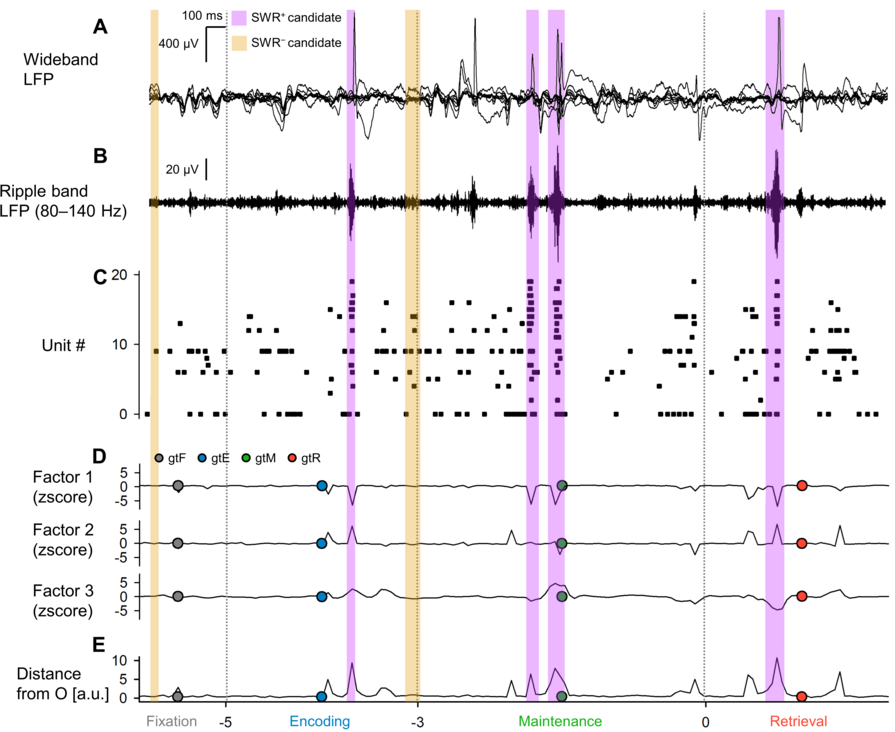
\includegraphics[width=1\textwidth]{./src/figures/.png/Figure_ID_01.png}
        	\caption{\textbf{
Local Field Potentials (LFP), Multiunit Activity, and Neural Trajectories in the Hippocampus During a Modified Sternberg Task
}
\smallskip
\\
\textbf{\textit{A.}} \DIFdelbeginFL \DIFdelFL{These }\DIFdelendFL \DIFaddbeginFL \DIFaddFL{The presented }\DIFaddendFL traces \DIFdelbeginFL \DIFdelFL{show }\DIFdelendFL \DIFaddbeginFL \DIFaddFL{illustrate }\DIFaddendFL representative wideband LFP intracranial EEG (iEEG) signals\DIFaddbeginFL \DIFaddFL{, }\DIFaddendFL recorded from the left hippocampal head \DIFdelbeginFL \DIFdelFL{. The }\DIFdelendFL \DIFaddbeginFL \DIFaddFL{while the }\DIFaddendFL subject \DIFdelbeginFL \DIFdelFL{performed }\DIFdelendFL \DIFaddbeginFL \DIFaddFL{was performing }\DIFaddendFL a modified Sternberg working memory task\DIFdelbeginFL \DIFdelFL{, which includes }\DIFdelendFL \DIFaddbeginFL \DIFaddFL{. This included phases of }\DIFaddendFL fixation (1 s, \textit{gray}), encoding (2 s, \textit{blue}), maintenance (3 s, \textit{green}), and retrieval (2 s, \textit{red}). \textbf{\textit{B.}} \DIFdelbeginFL \DIFdelFL{We then present }\DIFdelendFL \DIFaddbeginFL \DIFaddFL{Subsequently, }\DIFaddendFL the corresponding ripple band LFP traces \DIFaddbeginFL \DIFaddFL{are delineated}\DIFaddendFL . \textbf{\textit{C.}} The raster plot \DIFdelbeginFL \DIFdelFL{depicts }\DIFdelendFL \DIFaddbeginFL \DIFaddFL{represents }\DIFaddendFL multiunit spikes \DIFdelbeginFL \DIFdelFL{taken }\DIFdelendFL \DIFaddbeginFL \DIFaddFL{drawn }\DIFaddendFL from the LFP traces, sorted \DIFdelbeginFL \DIFdelFL{using }\DIFdelendFL \DIFaddbeginFL \DIFaddFL{by }\DIFaddendFL a \DIFdelbeginFL \DIFdelFL{spike }\DIFdelendFL \DIFaddbeginFL \DIFaddFL{reliable spike-sorting }\DIFaddendFL algorithm \cite{niediek_reliable_2016}. \textbf{\textit{D.}} \DIFdelbeginFL \DIFdelFL{Subsequently}\DIFdelendFL \DIFaddbeginFL \DIFaddFL{Following that}\DIFaddendFL , we \DIFdelbeginFL \DIFdelFL{illustrate }\DIFdelendFL \DIFaddbeginFL \DIFaddFL{portray }\DIFaddendFL the neural trajectories, which \DIFdelbeginFL \DIFdelFL{are calculated by }\DIFdelendFL \DIFaddbeginFL \DIFaddFL{have been computed using }\DIFaddendFL GPFA on spike counts per unit \DIFdelbeginFL \DIFdelFL{with }\DIFdelendFL \DIFaddbeginFL \DIFaddFL{within }\DIFaddendFL 50-ms bins. Each phase's geometric median is \DIFdelbeginFL \DIFdelFL{marked }\DIFdelendFL \DIFaddbeginFL \DIFaddFL{denoted }\DIFaddendFL by \DIFdelbeginFL \DIFdelFL{the }\DIFdelendFL dot circles. \textbf{\textit{E.}} The \DIFdelbeginFL \DIFdelFL{trajectory's }\DIFdelendFL distance \DIFaddbeginFL \DIFaddFL{of the trajectory }\DIFaddendFL from the origin $O$ is \DIFdelbeginFL \DIFdelFL{portrayed}\DIFdelendFL \DIFaddbeginFL \DIFaddFL{presented}\DIFaddendFL , with \textit{purple} and \textit{yellow} rectangles indicating the timings for SWR$^+$ candidates and SWR$^-$ candidates (\DIFdelbeginFL \DIFdelFL{considered }\DIFdelendFL \DIFaddbeginFL \DIFaddFL{acting }\DIFaddendFL as controls for SWR$^+$), respectively.
}
% width=1\textwidth
        	\label{fig:01}
        \end{figure*}
        \clearpage
        \begin{figure*}[ht]
            \pdfbookmark[2]{ID 02}{figure_id_02}
        	\centering
            \includegraphics[width=0.5\textwidth]{./src/figures/.png/Figure_ID_02.png}
        	\caption{\textbf{
State-Dependent Trajectories of Hippocampal Neurons
}
\smallskip
\\
\textbf{\textit{A.}} \DIFdelbeginFL \DIFdelFL{Neural }\DIFdelendFL \DIFaddbeginFL \DIFaddFL{This panel depicts neural }\DIFaddendFL trajectories within the \DIFdelbeginFL \DIFdelFL{initial }\DIFdelendFL \DIFaddbeginFL \DIFaddFL{first }\DIFaddendFL three-dimensional factors derived from \DIFdelbeginFL \DIFdelFL{the }\DIFdelendFL Gaussian Process Factor Analysis (GPFA)\DIFdelbeginFL \DIFdelFL{are displayed}\DIFdelendFL . \DIFdelbeginFL \DIFdelFL{The smaller }\DIFdelendFL \DIFaddbeginFL \DIFaddFL{Smaller }\DIFaddendFL dots \DIFdelbeginFL \DIFdelFL{correspond to }\DIFdelendFL \DIFaddbeginFL \DIFaddFL{represent }\DIFaddendFL coordinates \DIFdelbeginFL \DIFdelFL{of }\DIFdelendFL \DIFaddbeginFL \DIFaddFL{corresponding to }\DIFaddendFL 50-ms neural trajectory bins\DIFaddbeginFL \DIFaddFL{. Meanwhile}\DIFaddendFL , \DIFdelbeginFL \DIFdelFL{while the }\DIFdelendFL larger dots with \textit{black} \DIFdelbeginFL \DIFdelFL{edges signify the }\DIFdelendFL \DIFaddbeginFL \DIFaddFL{borders denote }\DIFaddendFL geometric medians for \DIFdelbeginFL \DIFdelFL{respective }\DIFdelendFL \DIFaddbeginFL \DIFaddFL{different }\DIFaddendFL stages in the Sternberg working memory task\DIFaddbeginFL \DIFaddFL{, as follows}\DIFaddendFL : fixation (\textit{gray}), encoding (\textit{blue}), maintenance (\textit{green}), and retrieval (\textit{red}). \textbf{\textit{B.}} The \DIFdelbeginFL \DIFdelFL{figure conveys }\DIFdelendFL \DIFaddbeginFL \DIFaddFL{graph presents }\DIFaddendFL the log-likelihood of the GPFA models \DIFdelbeginFL \DIFdelFL{versus }\DIFdelendFL \DIFaddbeginFL \DIFaddFL{compared with }\DIFaddendFL the \DIFdelbeginFL \DIFdelFL{count }\DIFdelendFL \DIFaddbeginFL \DIFaddFL{number }\DIFaddendFL of dimensions used to embed multiunit spikes \DIFdelbeginFL \DIFdelFL{found in }\DIFdelendFL \DIFaddbeginFL \DIFaddFL{from }\DIFaddendFL the medial temporal lobe (MTL) territories. \DIFdelbeginFL \DIFdelFL{In specific}\DIFdelendFL \DIFaddbeginFL \DIFaddFL{Specifically}\DIFaddendFL , the \DIFdelbeginFL \DIFdelFL{elbow method pinpointed the }\DIFdelendFL optimal dimension\DIFaddbeginFL \DIFaddFL{, as indicated by the elbow method, was found }\DIFaddendFL to be three. \textbf{\textit{C.}} This \DIFdelbeginFL \DIFdelFL{panel }\DIFdelendFL \DIFaddbeginFL \DIFaddFL{figure }\DIFaddendFL illustrates the distance of the neural trajectories from the origin ($O$) for the hippocampus (Hipp.), entorhinal cortex (EC), and amygdala (Amy.), \DIFdelbeginFL \DIFdelFL{against the }\DIFdelendFL \DIFaddbeginFL \DIFaddFL{over }\DIFaddendFL time \DIFdelbeginFL \DIFdelFL{elapsed from }\DIFdelendFL \DIFaddbeginFL \DIFaddFL{following }\DIFaddendFL the probe onset. \textbf{\textit{D.}} The \DIFdelbeginFL \DIFdelFL{distance }\DIFdelendFL \DIFaddbeginFL \DIFaddFL{panel displays distances }\DIFaddendFL of the \DIFdelbeginFL \DIFdelFL{trajectory }\DIFdelendFL \DIFaddbeginFL \DIFaddFL{trajectories }\DIFaddendFL from $O$ within \DIFaddbeginFL \DIFaddFL{the }\DIFaddendFL MTL \DIFdelbeginFL \DIFdelFL{regions is displayed}\DIFdelendFL \DIFaddbeginFL \DIFaddFL{areas}\DIFaddendFL . The hippocampus \DIFdelbeginFL \DIFdelFL{shows }\DIFdelendFL \DIFaddbeginFL \DIFaddFL{demonstrates }\DIFaddendFL the \DIFdelbeginFL \DIFdelFL{farthest }\DIFdelendFL \DIFaddbeginFL \DIFaddFL{greatest }\DIFaddendFL distance, followed by the EC and the Amygdala. \textbf{\textit{E.}} \DIFdelbeginFL \DIFdelFL{The plot represents inter-phase trajectory }\DIFdelendFL \DIFaddbeginFL \DIFaddFL{This graph displays the }\DIFaddendFL distances \DIFaddbeginFL \DIFaddFL{between phases of the trajectories }\DIFaddendFL within the MTL regions.
Abbreviations:
}
% width=0.5\textwidth
        	\label{fig:02}
        \end{figure*}
        \clearpage
        \begin{figure*}[ht]
            \pdfbookmark[2]{ID 03}{figure_id_03}
        	\centering
            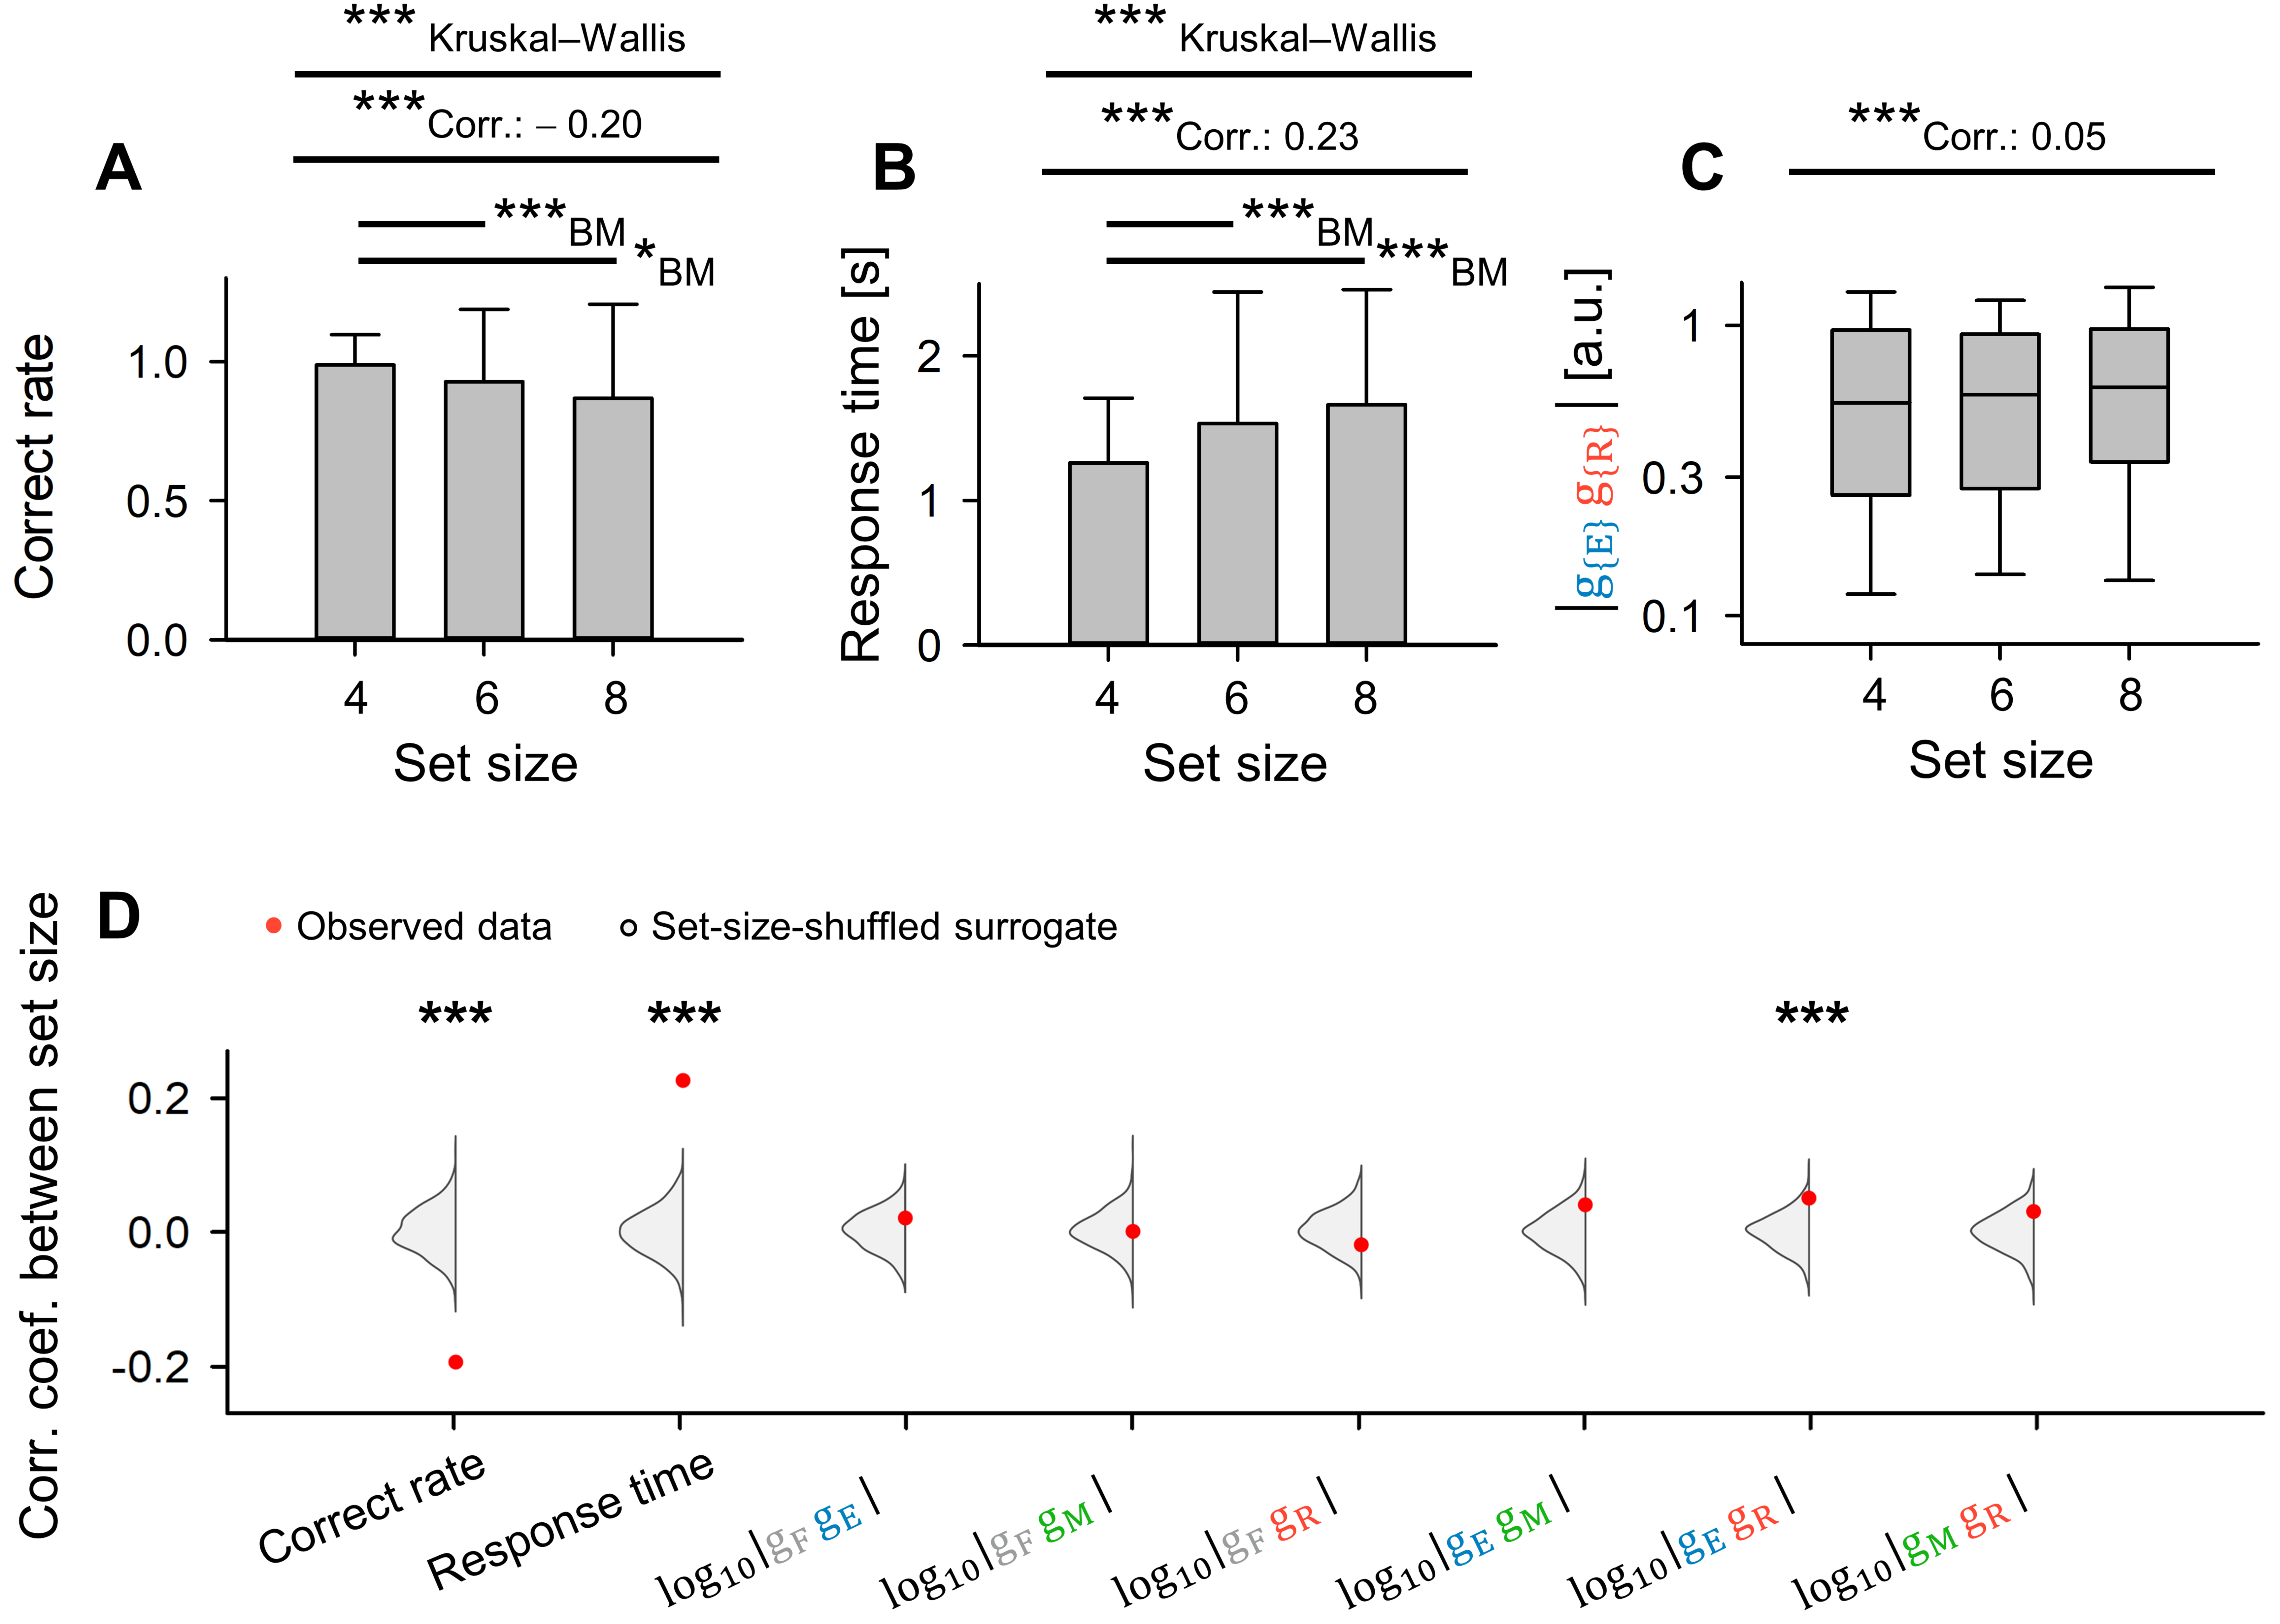
\includegraphics[width=1\textwidth]{./src/figures/.png/Figure_ID_03.png}
        	\caption{\DIFdelbeginFL \textbf{\DIFdelFL{Dependency of Trajectory Distance on Memory Load: Encoding and Retrieval States in Hippocampus
}}
%DIFAUXCMD
\DIFdelendFL \DIFaddbeginFL \textbf{
\DIFaddFL{Dependency of Trajectory Distance on Memory Load: Encoding and Retrieval States in the Hippocampus.
}}
\DIFaddendFL \smallskip
\\
\textbf{\textit{A.}} \DIFdelbeginFL \DIFdelFL{The }\DIFdelendFL \DIFaddbeginFL \DIFaddFL{Illustrates the }\DIFaddendFL relationship between set size (\DIFaddbeginFL \DIFaddFL{the }\DIFaddendFL number of letters that \DIFdelbeginFL \DIFdelFL{need to be encoded}\DIFdelendFL \DIFaddbeginFL \DIFaddFL{require encoding}\DIFaddendFL ) and \DIFaddbeginFL \DIFaddFL{the }\DIFaddendFL correct rate in the working memory task (coefficient = $-0.20$, ***\textit{p} $<$ 0.001). \textbf{\textit{B.}} \DIFdelbeginFL \DIFdelFL{The }\DIFdelendFL \DIFaddbeginFL \DIFaddFL{Showcases the }\DIFaddendFL correlation between set size and response time (coefficient = 0.23, ***\textit{p} $<$ 0.001). \textbf{\textit{C.}} \DIFdelbeginFL \DIFdelFL{The impact }\DIFdelendFL \DIFaddbeginFL \DIFaddFL{Depicts the influence }\DIFaddendFL of set size on the inter-phase distances between the encoding and retrieval phases ($\lVert \mathrm{g_{E}g_{R}} \rVert$) (correlation coefficient = 0.05). \textbf{\textit{D.}} \textit{Red} dots represent experimental observations of correlations between set size and the \DIFdelbeginFL \DIFdelFL{following }\DIFdelendFL \DIFaddbeginFL \DIFaddFL{ensuing }\DIFaddendFL parameters: correct rate, response time, $\log_{10}{\lVert \mathrm{g_{F}g_{E}} \rVert}$, $\log_{10}{\lVert \mathrm{g_{F}g_{M}} \rVert}$, $\log_{10}{\lVert \mathrm{g_{F}g_{R}} \rVert}$, $\log_{10}{\lVert \mathrm{g_{E}g_{M}} \rVert}$, $\log_{10}{\lVert \mathrm{g_{E}g_{R}} \rVert}$, and $\log_{10}{\lVert \mathrm{g_{M}g_{R}} \rVert}$. The \textit{gray} kernel density plot \DIFdelbeginFL \DIFdelFL{illustrates }\DIFdelendFL \DIFaddbeginFL \DIFaddFL{demonstrates }\DIFaddendFL the corresponding set-size-shuffled surrogate (\textit{n} = 1,000) (***\textit{p}s $<$ 0.001).
}
% width=1\textwidth
        	\label{fig:03}
        \end{figure*}
        \clearpage
        \begin{figure*}[ht]
            \pdfbookmark[2]{ID 04}{figure_id_04}
        	\centering
            \includegraphics[width=1\textwidth]{./src/figures/.png/Figure_ID_04.png}
        	\caption{\DIFdelbeginFL \textbf{\DIFdelFL{Detection of SWRs in Presumptive CA1 Regions
}}
%DIFAUXCMD
\DIFdelendFL \DIFaddbeginFL \textbf{
\DIFaddFL{Detection of SWRs in Prospective CA1 Regions
}}
\DIFaddendFL \smallskip
\\
\textbf{\textit{A.}} \DIFdelbeginFL \DIFdelFL{Two-dimensional }\DIFdelendFL \DIFaddbeginFL \DIFaddFL{A two-dimensional }\DIFaddendFL UMAP (Uniform Manifold Approximation and Projection) \cite{mcinnes_umap_2018} projection \DIFdelbeginFL \DIFdelFL{of }\DIFdelendFL \DIFaddbeginFL \DIFaddFL{that utilizes }\DIFaddendFL multiunit spikes \DIFaddbeginFL \DIFaddFL{is presented }\DIFaddendFL during SWR$^+$ candidates (\textit{purple}) and SWR$^-$ candidates (\textit{yellow}). \textbf{\textit{B.}} \DIFdelbeginFL \DIFdelFL{Cumulative }\DIFdelendFL \DIFaddbeginFL \DIFaddFL{A cumulative }\DIFaddendFL density plot \DIFdelbeginFL \DIFdelFL{shows }\DIFdelendFL \DIFaddbeginFL \DIFaddFL{displaying }\DIFaddendFL silhouette scores, indicative of \DIFaddbeginFL \DIFaddFL{the }\DIFaddendFL UMAP clustering quality, \DIFaddbeginFL \DIFaddFL{is provided }\DIFaddendFL for hippocampal regions (\DIFdelbeginFL \DIFdelFL{see }\DIFdelendFL Table~\ref{tab:02} \DIFdelbeginFL \DIFdelFL{for }\DIFdelendFL \DIFaddbeginFL \DIFaddFL{as }\DIFaddendFL reference). \DIFdelbeginFL \DIFdelFL{Note that hippocampal }\DIFdelendFL \DIFaddbeginFL \DIFaddFL{Hippocampal }\DIFaddendFL regions \DIFdelbeginFL \DIFdelFL{with }\DIFdelendFL \DIFaddbeginFL \DIFaddFL{that exhibit }\DIFaddendFL silhouette scores greater than 0.60\DIFdelbeginFL \DIFdelFL{(}\DIFdelendFL \DIFaddbeginFL \DIFaddFL{, }\DIFaddendFL equivalent to the $75^{th}$ percentile\DIFdelbeginFL \DIFdelFL{) were }\DIFdelendFL \DIFaddbeginFL \DIFaddFL{, are }\DIFaddendFL identified as \DIFdelbeginFL \DIFdelFL{possible }\DIFdelendFL \DIFaddbeginFL \DIFaddFL{probable }\DIFaddendFL CA1 regions. SWR$^+$ and SWR$^-$ candidates \DIFdelbeginFL \DIFdelFL{recorded }\DIFdelendFL \DIFaddbeginFL \DIFaddFL{obtained }\DIFaddendFL from these \DIFdelbeginFL \DIFdelFL{speculative }\DIFdelendFL \DIFaddbeginFL \DIFaddFL{hypothetical }\DIFaddendFL CA1 regions \DIFdelbeginFL \DIFdelFL{were }\DIFdelendFL \DIFaddbeginFL \DIFaddFL{are }\DIFaddendFL respectively \DIFdelbeginFL \DIFdelFL{classified }\DIFdelendFL \DIFaddbeginFL \DIFaddFL{categorized }\DIFaddendFL as SWR$^+$ and SWR$^-$ (\DIFaddbeginFL \DIFaddFL{with }\DIFaddendFL \textit{n}s = 1,170). \textbf{\textit{C.}} The \DIFdelbeginFL \DIFdelFL{identical }\DIFdelendFL \DIFaddbeginFL \DIFaddFL{same }\DIFaddendFL distributions of durations are presented for \DIFaddbeginFL \DIFaddFL{both }\DIFaddendFL SWR$^+$ (\textit{purple}) and SWR$^-$ (\textit{yellow}) \DIFdelbeginFL \DIFdelFL{, owing }\DIFdelendFL \DIFaddbeginFL \DIFaddFL{due }\DIFaddendFL to their \DIFdelbeginFL \DIFdelFL{definitions }\DIFdelendFL \DIFaddbeginFL \DIFaddFL{similar natures }\DIFaddendFL (93.0 [65.4] ms, \DIFaddbeginFL \DIFaddFL{expressed as }\DIFaddendFL median [IQR]). \textbf{\textit{D.}} \DIFaddbeginFL \DIFaddFL{An illustration of the }\DIFaddendFL SWR incidence for both \DIFaddbeginFL \DIFaddFL{the }\DIFaddendFL SWR$^+$ (\textit{purple}) and SWR$^-$ (\textit{yellow}) \DIFdelbeginFL \DIFdelFL{obtained }\DIFdelendFL relative to the probe's timing is \DIFdelbeginFL \DIFdelFL{illustrated }\DIFdelendFL \DIFaddbeginFL \DIFaddFL{conveyed }\DIFaddendFL as a mean \DIFdelbeginFL %DIFDELCMD < \textpm %%%
\DIFdelendFL \DIFaddbeginFL \DIFaddFL{with a }\DIFaddendFL 95\% confidence interval. However, \DIFdelbeginFL \DIFdelFL{as }\DIFdelendFL \DIFaddbeginFL \DIFaddFL{given that }\DIFaddendFL the intervals may not be \DIFdelbeginFL \DIFdelFL{visible }\DIFdelendFL \DIFaddbeginFL \DIFaddFL{noticeable }\DIFaddendFL due to their \DIFdelbeginFL \DIFdelFL{narrow }\DIFdelendFL \DIFaddbeginFL \DIFaddFL{slender }\DIFaddendFL range, \DIFdelbeginFL \DIFdelFL{note }\DIFdelendFL \DIFaddbeginFL \DIFaddFL{it should be highlighted }\DIFaddendFL that a significant \DIFdelbeginFL \DIFdelFL{increase }\DIFdelendFL \DIFaddbeginFL \DIFaddFL{rise }\DIFaddendFL in SWR incidence was \DIFdelbeginFL \DIFdelFL{detected }\DIFdelendFL \DIFaddbeginFL \DIFaddFL{discovered }\DIFaddendFL during the \DIFdelbeginFL \DIFdelFL{initial }\DIFdelendFL \DIFaddbeginFL \DIFaddFL{beginning }\DIFaddendFL 400 ms of the retrieval phase (0.421 [Hz], *\textit{p} $<$ 0.05, \DIFaddbeginFL \DIFaddFL{verified by a }\DIFaddendFL bootstrap test). \textbf{\textit{E.}} The distributions of ripple band peak amplitudes for SWR$^-$ (\textit{yellow}; 2.37 [0.33] SD of baseline, median [IQR]) and SWR$^+$ (\textit{purple}; 3.05 [0.85] SD of baseline, median [IQR]) are \DIFdelbeginFL \DIFdelFL{delineated }\DIFdelendFL \DIFaddbeginFL \DIFaddFL{outlined }\DIFaddendFL (***\textit{p} $<$ 0.001, \DIFaddbeginFL \DIFaddFL{confirmed by }\DIFaddendFL the Brunner--Munzel test).
}
% width=1\textwidth
        	\label{fig:04}
        \end{figure*}
        \clearpage
        \begin{figure*}[ht]
            \pdfbookmark[2]{ID 05}{figure_id_05}
        	\centering
            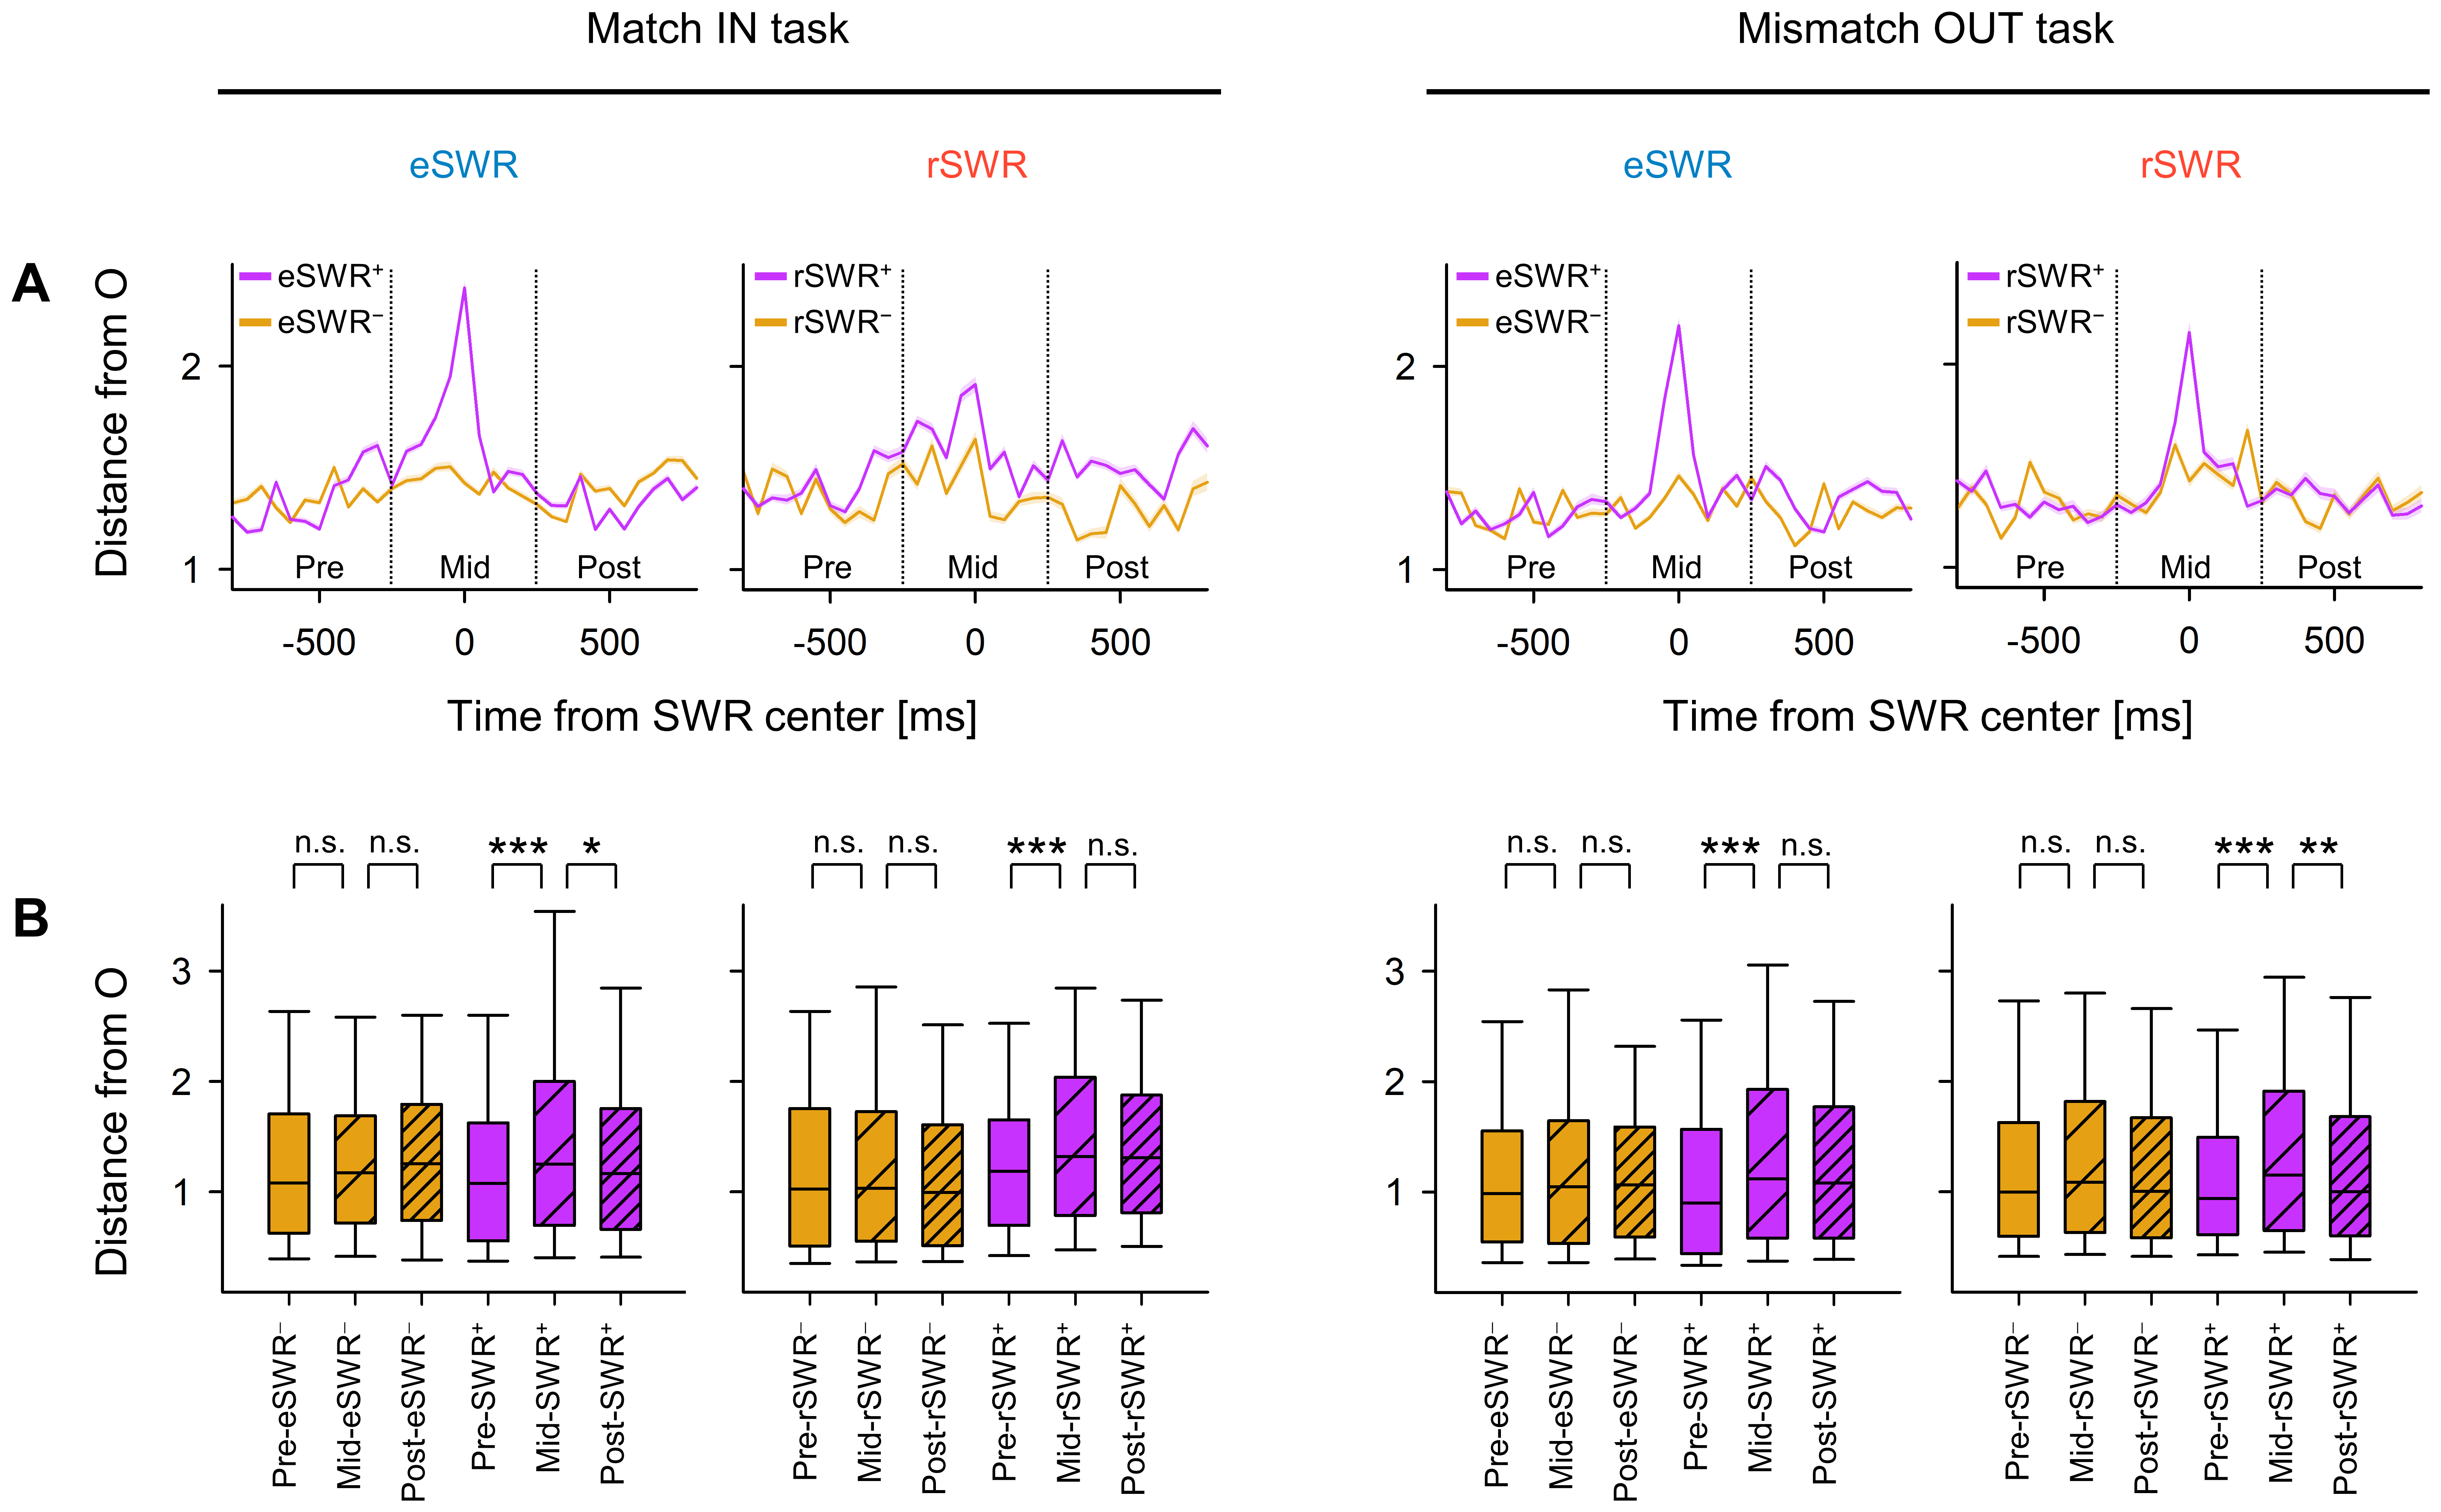
\includegraphics[width=1\textwidth]{./src/figures/.png/Figure_ID_05.png}
        	\caption{\DIFdelbeginFL \textbf{\DIFdelFL{Transient Alterations in Neural Trajectory During SWR Events
}}
%DIFAUXCMD
\DIFdelendFL \DIFaddbeginFL \textbf{
\DIFaddFL{Transient Changes in Neural Trajectory During SWR Events
}}
\DIFaddendFL \smallskip
\\
\textbf{\textit{A.}} \DIFdelbeginFL \DIFdelFL{Displayed }\DIFdelendFL \DIFaddbeginFL \DIFaddFL{Depicted }\DIFaddendFL is the distance from \DIFaddbeginFL \DIFaddFL{the }\DIFaddendFL origin ($O$) of the peri-sharp-wave-ripple \DIFdelbeginFL \DIFdelFL{trajectory }\DIFdelendFL (\DIFaddbeginFL \DIFaddFL{SWR) trajectory, calculated as the }\DIFaddendFL mean \textpm 95\% confidence interval\DIFdelbeginFL \DIFdelFL{)}\DIFdelendFL . The intervals \DIFdelbeginFL \DIFdelFL{may }\DIFdelendFL \DIFaddbeginFL \DIFaddFL{might }\DIFaddendFL not be \DIFdelbeginFL \DIFdelFL{apparent }\DIFdelendFL \DIFaddbeginFL \DIFaddFL{noticeable }\DIFaddendFL due to their \DIFdelbeginFL \DIFdelFL{slender ranges}\DIFdelendFL \DIFaddbeginFL \DIFaddFL{narrow magnitudes}\DIFaddendFL . \textbf{\textit{B.}} \DIFdelbeginFL \DIFdelFL{Shown }\DIFdelendFL \DIFaddbeginFL \DIFaddFL{Illustrated }\DIFaddendFL is the distance from the origin ($O$) during \DIFaddbeginFL \DIFaddFL{the }\DIFaddendFL pre-, mid-, and post-SWR \DIFdelbeginFL \DIFdelFL{periods }\DIFdelendFL \DIFaddbeginFL \DIFaddFL{phases }\DIFaddendFL (*\textit{p} $<$ 0.05, **\textit{p} $<$ 0.01, ***\textit{p} $<$ 0.001; \DIFdelbeginFL \DIFdelFL{assessed }\DIFdelendFL \DIFaddbeginFL \DIFaddFL{evaluated }\DIFaddendFL using the Brunner--Munzel test). Abbreviations: SWR, sharp-wave ripple events; eSWR, SWR \DIFdelbeginFL \DIFdelFL{during }\DIFdelendFL \DIFaddbeginFL \DIFaddFL{within }\DIFaddendFL the encoding phase; rSWR, SWR \DIFdelbeginFL \DIFdelFL{while in the }\DIFdelendFL \DIFaddbeginFL \DIFaddFL{during }\DIFaddendFL retrieval phase; SWR$^+$, positive SWR event; SWR$^-$, control events for SWR$^+$; pre-, mid-, or post-SWR \DIFdelbeginFL \DIFdelFL{denote }\DIFdelendFL \DIFaddbeginFL \DIFaddFL{refer to }\DIFaddendFL the time intervals from $-800$ to $-250$ ms, from $-250$ to $+250$ ms, or from $+250$ to $+800$ ms, all \DIFdelbeginFL \DIFdelFL{relative }\DIFdelendFL \DIFaddbeginFL \DIFaddFL{in relation }\DIFaddendFL to the \DIFdelbeginFL \DIFdelFL{center }\DIFdelendFL \DIFaddbeginFL \DIFaddFL{central point }\DIFaddendFL of the SWR.
}
% width=1\textwidth
        	\label{fig:05}
        \end{figure*}
        \clearpage
        \begin{figure*}[ht]
            \pdfbookmark[2]{ID 06}{figure_id_06}
        	\centering
            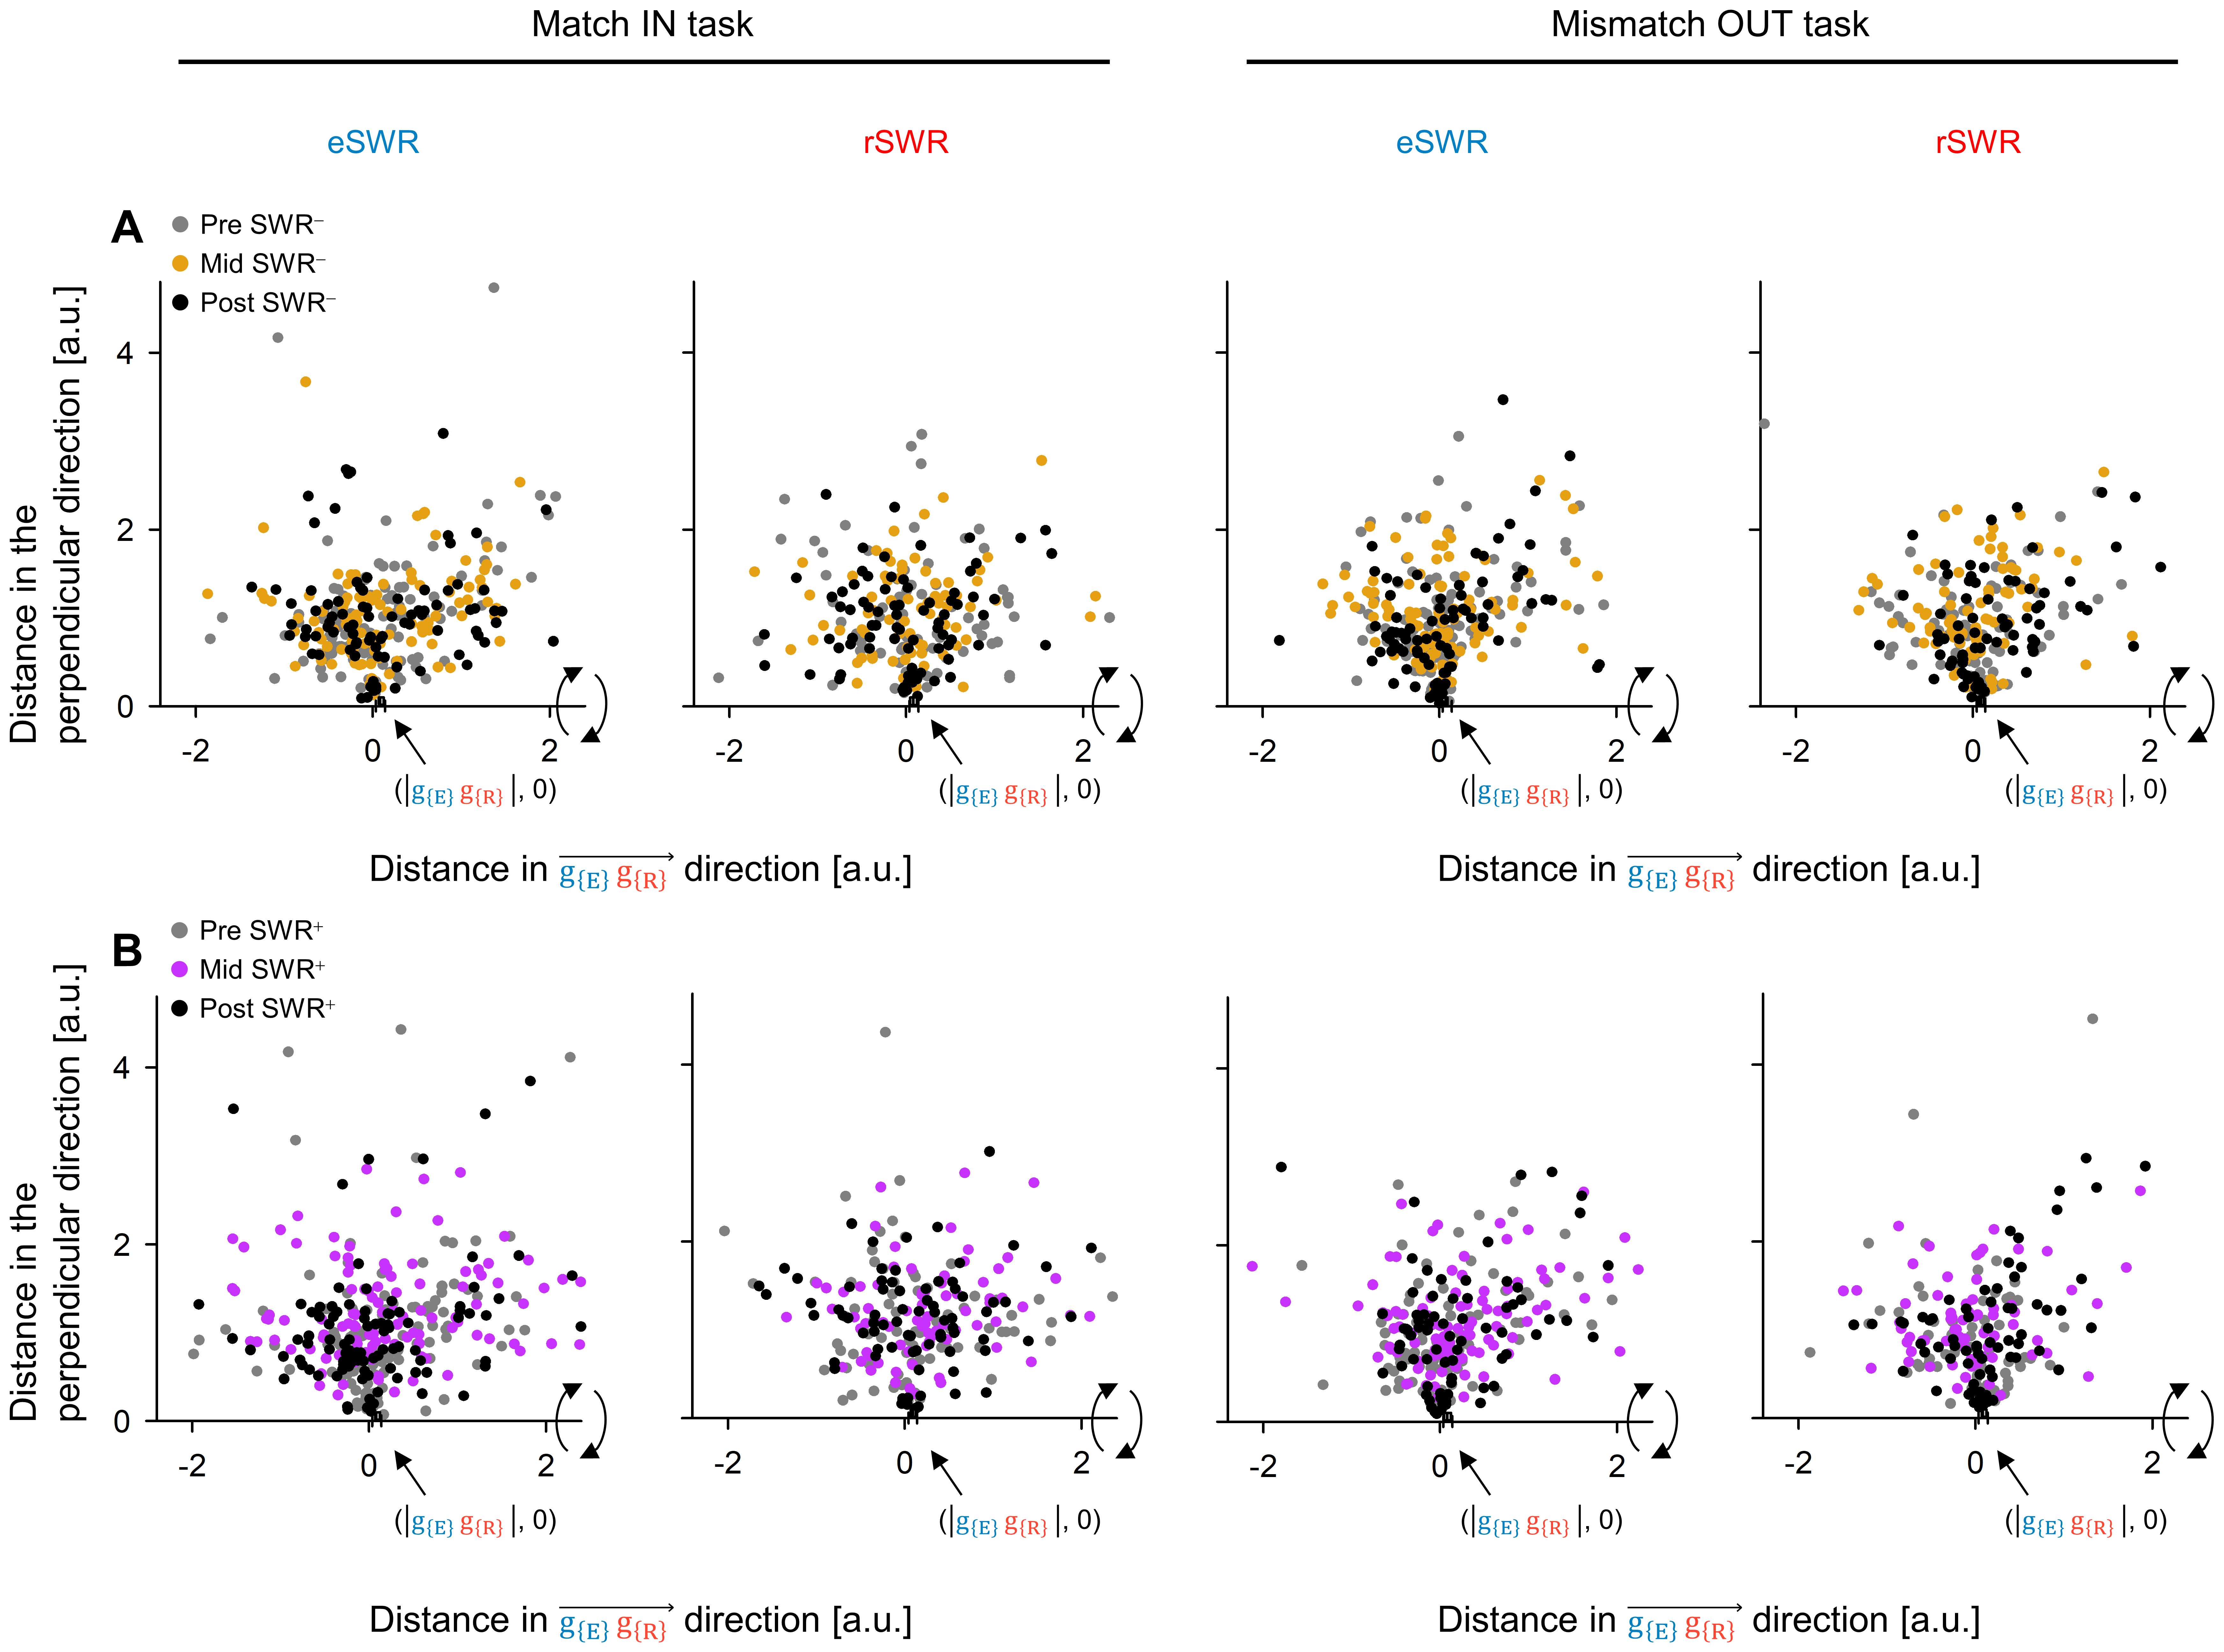
\includegraphics[width=1\textwidth]{./src/figures/.png/Figure_ID_06.png}
        	\caption{\DIFdelbeginFL \textbf{\DIFdelFL{Visualization of Neural Trajectories during SWR in Two-Dimensional Spaces}}
%DIFAUXCMD
\DIFdelendFL \DIFaddbeginFL \textbf{
\DIFaddFL{Visualizing Neural Trajectories during SWR in Two-Dimensional Spaces}}
\DIFaddendFL \smallskip
\\
The \DIFdelbeginFL \DIFdelFL{panels display }\DIFdelendFL \DIFaddbeginFL \DIFaddFL{figures depict }\DIFaddendFL hippocampal neural trajectories during SWR\DIFdelbeginFL \DIFdelFL{as }\DIFdelendFL \DIFaddbeginFL \DIFaddFL{, }\DIFaddendFL projected onto two-dimensional spaces. \textbf{\textit{A.}} \DIFdelbeginFL \DIFdelFL{Indicates }\DIFdelendFL \DIFaddbeginFL \DIFaddFL{Displays }\DIFaddendFL hippocampal neural trajectories \DIFdelbeginFL \DIFdelFL{pre-SWR$^-$ }\DIFdelendFL \DIFaddbeginFL \DIFaddFL{before }\DIFaddendFL (\DIFdelbeginFL \textit{\DIFdelFL{gray}}%DIFAUXCMD
\DIFdelendFL \DIFaddbeginFL \DIFaddFL{pre}\DIFaddendFL ), \DIFdelbeginFL \DIFdelFL{mid-SWR$^-$ }\DIFdelendFL \DIFaddbeginFL \DIFaddFL{during }\DIFaddendFL (\DIFdelbeginFL \textit{\DIFdelFL{yellow}}%DIFAUXCMD
\DIFdelendFL \DIFaddbeginFL \DIFaddFL{mid}\DIFaddendFL ), and \DIFdelbeginFL \DIFdelFL{post-SWR$^-$ }\DIFdelendFL \DIFaddbeginFL \DIFaddFL{after }\DIFaddendFL (\DIFdelbeginFL \textit{\DIFdelFL{black}}%DIFAUXCMD
\DIFdelendFL \DIFaddbeginFL \DIFaddFL{post}\DIFaddendFL ) \DIFaddbeginFL \DIFaddFL{SWR$^-$, denoted in }\textit{\DIFaddFL{gray}}\DIFaddFL{, }\textit{\DIFaddFL{yellow}}\DIFaddFL{, and }\textit{\DIFaddFL{black}}\DIFaddFL{, respectively}\DIFaddendFL . \textbf{\textit{B.}} \DIFdelbeginFL \DIFdelFL{Represents }\DIFdelendFL \DIFaddbeginFL \DIFaddFL{Shows }\DIFaddendFL the \DIFdelbeginFL \DIFdelFL{equivalents }\DIFdelendFL \DIFaddbeginFL \DIFaddFL{corresponding trajectories }\DIFaddendFL for SWR$^+$\DIFdelbeginFL \DIFdelFL{as opposed to SWR$^-$}\DIFdelendFL . The \DIFaddbeginFL \DIFaddFL{magnitude of }\DIFaddendFL $\lVert \mathrm{g_{E}g_{R}} \rVert$ varied \DIFdelbeginFL \DIFdelFL{among }\DIFdelendFL \DIFaddbeginFL \DIFaddFL{across }\DIFaddendFL sessions. The \DIFaddbeginFL \DIFaddFL{following }\DIFaddendFL projection \DIFaddbeginFL \DIFaddFL{method }\DIFaddendFL was \DIFdelbeginFL \DIFdelFL{applied in the following manner}\DIFdelendFL \DIFaddbeginFL \DIFaddFL{employed}\DIFaddendFL : \DIFdelbeginFL \DIFdelFL{First}\DIFdelendFL \DIFaddbeginFL \DIFaddFL{Firstly}\DIFaddendFL , a linear transformation positioned $\mathrm{g_{E}}$ at \DIFdelbeginFL \DIFdelFL{the }\DIFdelendFL origin $O$ (0,0), and $\mathrm{g_{R}}$ at ($\lVert \mathrm{g_{E}g_{R}} \rVert$, 0). The point cloud was then rotated around the $\mathrm{g_{E}g_{R}}$ axis (\DIFdelbeginFL \DIFdelFL{equivalent }\DIFdelendFL \DIFaddbeginFL \DIFaddFL{identical }\DIFaddendFL to the \DIFdelbeginFL \DIFdelFL{x axis}\DIFdelendFL \DIFaddbeginFL \DIFaddFL{x-axis}\DIFaddendFL ) \DIFdelbeginFL \DIFdelFL{for fitting }\DIFdelendFL \DIFaddbeginFL \DIFaddFL{to fit }\DIFaddendFL into \DIFaddbeginFL \DIFaddFL{the }\DIFaddendFL two-dimensional spaces. \DIFdelbeginFL \DIFdelFL{Therefore}\DIFdelendFL \DIFaddbeginFL \DIFaddFL{Consequently}\DIFaddendFL , within these two-dimensional spaces, \DIFdelbeginFL \DIFdelFL{both }\DIFdelendFL the distances from $O$ and the angles \DIFdelbeginFL \DIFdelFL{preserved }\DIFdelendFL \DIFaddbeginFL \DIFaddFL{remained consistent with }\DIFaddendFL the original \DIFdelbeginFL \DIFdelFL{makeup }\DIFdelendFL \DIFaddbeginFL \DIFaddFL{properties }\DIFaddendFL of the $\mathrm{g_{E}g_{R}}$ axis \DIFdelbeginFL \DIFdelFL{from }\DIFdelendFL \DIFaddbeginFL \DIFaddFL{in }\DIFaddendFL the \DIFdelbeginFL \DIFdelFL{original }\DIFdelendFL three-dimensional spaces. Abbreviations: SWR \DIFdelbeginFL \DIFdelFL{signifies }\DIFdelendFL \DIFaddbeginFL \DIFaddFL{refers to }\DIFaddendFL sharp-wave ripple events; eSWR \DIFdelbeginFL \DIFdelFL{denotes }\DIFdelendFL \DIFaddbeginFL \DIFaddFL{represents }\DIFaddendFL SWR during the encoding phase; rSWR \DIFdelbeginFL \DIFdelFL{indicates }\DIFdelendFL \DIFaddbeginFL \DIFaddFL{denotes }\DIFaddendFL SWR during \DIFdelbeginFL \DIFdelFL{the }\DIFdelendFL retrieval phase; SWR$^+$ \DIFdelbeginFL \DIFdelFL{, marks }\DIFdelendFL \DIFaddbeginFL \DIFaddFL{indicates }\DIFaddendFL an \DIFaddbeginFL \DIFaddFL{occurrence of }\DIFaddendFL SWR event; SWR$^-$ refers to control events for SWR$^+$; pre-SWR, mid-SWR, or post-SWR \DIFdelbeginFL \DIFdelFL{, reference the }\DIFdelendFL \DIFaddbeginFL \DIFaddFL{refer to }\DIFaddendFL time intervals from $-800$ to $-250$ ms, from $-250$ to $+250$ ms, or from $+250$ to $+800$ ms from the center of SWR\DIFaddbeginFL \DIFaddFL{, respectively}\DIFaddendFL .}
% width=1\textwidth
        	\label{fig:06}
        \end{figure*}
        \clearpage
        \begin{figure*}[ht]
            \pdfbookmark[2]{ID 07}{figure_id_07}
        	\centering
            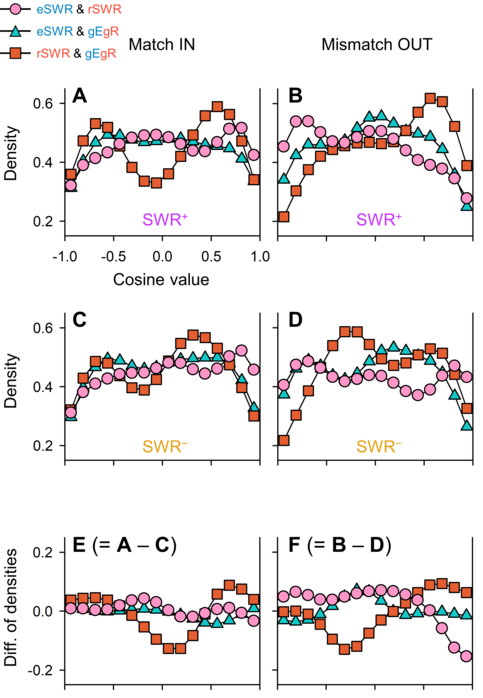
\includegraphics[width=0.5\textwidth]{./src/figures/.png/Figure_ID_07.png}
        	\caption{\DIFdelbeginFL \textbf{\DIFdelFL{Directions of Neural Trajectories during SWRs Based on Encoding and Retrieval States
}}
%DIFAUXCMD
\DIFdelendFL \DIFaddbeginFL \textbf{
\DIFaddFL{Neural Trajectory Directions during SWRs: Encoding and Retrieval States
}}
\DIFaddendFL \smallskip
\\
\textbf{\textit{A--B}} Kernel density estimation (KDE) distributions of $\protect\overrightarrow{{\mathrm{eSWR^+}}} \cdot \protect\overrightarrow{{\mathrm{rSWR^+}}}$ (\textit{pink circles}), $\protect\overrightarrow{{\mathrm{eSWR^+}}} \cdot \protect\overrightarrow{{\mathrm{g_{E}g_{R}}}}$ (\textit{blue triangles}), and $\protect\overrightarrow{{\mathrm{rSWR^+}}} \cdot \protect\overrightarrow{{\mathrm{g_{E}g_{R}}}}$ (\textit{red rectangles}) \DIFdelbeginFL \DIFdelFL{in }\DIFdelendFL \DIFaddbeginFL \DIFaddFL{are shown for }\DIFaddendFL Match \DIFdelbeginFL \DIFdelFL{In }\DIFdelendFL \DIFaddbeginFL \DIFaddFL{IN }\DIFaddendFL (\textit{A}) and Mismatch OUT tasks (\textit{B}). \textbf{\textit{C--D}} \DIFdelbeginFL \DIFdelFL{Present }\DIFdelendFL \DIFaddbeginFL \DIFaddFL{Display }\DIFaddendFL the corresponding distributions of $\mathrm{SWR^-}$ \DIFdelbeginFL \DIFdelFL{instead of }\DIFdelendFL \DIFaddbeginFL \DIFaddFL{replacing }\DIFaddendFL those of $\mathrm{SWR^+}$ in \textit{A} and \textit{B}. \textbf{\textit{E--F}} \DIFdelbeginFL \DIFdelFL{Depict }\DIFdelendFL \DIFaddbeginFL \DIFaddFL{Illustrate }\DIFaddendFL the \DIFdelbeginFL \DIFdelFL{differences }\DIFdelendFL \DIFaddbeginFL \DIFaddFL{discrepancies }\DIFaddendFL in the distributions of $\mathrm{SWR^+}$ and $\mathrm{SWR^-}$, \DIFdelbeginFL \DIFdelFL{illuminating }\DIFdelendFL \DIFaddbeginFL \DIFaddFL{highlighting }\DIFaddendFL the SWR components (\textit{E} = \textit{C} $-$ \textit{A}; \textit{F} = \textit{D} $-$ \textit{B}). \DIFdelbeginFL \DIFdelFL{Note }\DIFdelendFL \DIFaddbeginFL \DIFaddFL{Observe }\DIFaddendFL the biphasic distributions of $\protect\overrightarrow{{\mathrm{rSWR^-}}} \cdot \protect\overrightarrow{{\mathrm{g_{E}g_{R}}}}$, \DIFdelbeginFL \DIFdelFL{suggesting }\DIFdelendFL \DIFaddbeginFL \DIFaddFL{indicating }\DIFaddendFL fluctuations between the encoding and retrieval states \DIFdelbeginFL \DIFdelFL{during }\DIFdelendFL \DIFaddbeginFL \DIFaddFL{throughout }\DIFaddendFL the Sternberg task. \DIFdelbeginFL \DIFdelFL{Moreover}\DIFdelendFL \DIFaddbeginFL \DIFaddFL{Additionally}\DIFaddendFL , \DIFdelbeginFL \DIFdelFL{inverse }\DIFdelendFL \DIFaddbeginFL \DIFaddFL{contrasting }\DIFaddendFL directionality between $\protect\overrightarrow{{\mathrm{eSWR^+}}}$ and $\protect\overrightarrow{{\mathrm{rSWR^+}}}$ was \DIFdelbeginFL \DIFdelFL{observed }\DIFdelendFL \DIFaddbeginFL \DIFaddFL{noticed }\DIFaddendFL (\textit{pink circles}) in the Mismatch OUT task, but \DIFdelbeginFL \DIFdelFL{not }\DIFdelendFL \DIFaddbeginFL \DIFaddFL{was absent }\DIFaddendFL in the Match IN task \DIFaddbeginFL \DIFaddFL{(}\DIFaddendFL \textbf{\textit{E--F}}). \DIFdelbeginFL \DIFdelFL{Finally}\DIFdelendFL \DIFaddbeginFL \DIFaddFL{Lastly}\DIFaddendFL , \DIFdelbeginFL \DIFdelFL{shifts }\DIFdelendFL \DIFaddbeginFL \DIFaddFL{transitions }\DIFaddendFL from the retrieval to \DIFaddbeginFL \DIFaddFL{the }\DIFaddendFL encoding states were \DIFdelbeginFL \DIFdelFL{evident }\DIFdelendFL \DIFaddbeginFL \DIFaddFL{prominent }\DIFaddendFL in the SWR components in both the Match IN and Mismatch OUT tasks (\textit{red rectangles} in \textit{E} and \textit{F}).
}
% width=0.5\textwidth
        	\label{fig:07}
        \end{figure*}

%%%%%%%%%%%%%%%%%%%%%%%%%%%%%%%%%%%%%%%%%%%%%%%%%%%%%%%%%%%%%%%%%%%%%%%%%%%%%%%%
%% END
%%%%%%%%%%%%%%%%%%%%%%%%%%%%%%%%%%%%%%%%%%%%%%%%%%%%%%%%%%%%%%%%%%%%%%%%%%%%%%%%

\end{document}
